% ============================================================
%  宽松风险平价答辩 PPT  ·  ~50 页  ·  图片为主
%  编译：xelatex rrp_defense.tex  →  rrp_defense.pdf
%  图片路径：../results/figures/
% ============================================================
\documentclass[aspectratio=169,11pt]{beamer}
\usepackage{beamerthemeSWUFE}
\usepackage{booktabs}
\usepackage{amsmath}
\usepackage{array}
\usepackage{colortbl}

\graphicspath{{../results/figures/}{assets/logos/}}

% ── 封面信息 ──────────────────────────────────────────────────────────────────
\title{宽松风险平价在全球 ETF\\资产配置中的改进与实证研究}
\subtitle{本科毕业论文答辩}
\author{许哲圣}
\studentid{42353012}
\school{特拉华数据科学学院}
\major{金融数学（金融服务与量化分析方向）}
\supervisor{王磊 讲师}
\date{2026年5月}

% ── 数值宏（来自 generated_numbers.tex）─────────────────────────────────────
\newcommand{\etfCount}{30}
\newcommand{\evalStartDate}{2019-01-01}
\newcommand{\evalEndDate}{2026-05-29}
\newcommand{\evalMonths}{89}
\newcommand{\txCostBps}{3}
\newcommand{\riskFreeRate}{1.82\%}
\newcommand{\dataFirstDate}{2018-02-28}
\newcommand{\globalNetReturn}{4.59\%}
\newcommand{\globalSharpe}{0.674}
\newcommand{\globalMaxDD}{-7.14\%}
\newcommand{\globalMonthlyTurnover}{22.30\%}
\newcommand{\convexNetReturn}{6.80\%}
\newcommand{\convexSharpe}{0.956}
\newcommand{\convexMaxDD}{-6.66\%}
\newcommand{\convexMonthlyTurnover}{1.24\%}
\newcommand{\improvedNetReturn}{5.57\%}
\newcommand{\improvedVolatility}{2.62\%}
\newcommand{\improvedSharpe}{1.431}
\newcommand{\improvedSortino}{2.099}
\newcommand{\improvedMaxDD}{-3.95\%}
\newcommand{\improvedCalmar}{1.410}
\newcommand{\improvedMonthlyTurnover}{2.07\%}
\newcommand{\hercNetReturn}{2.23\%}
\newcommand{\hercSharpe}{0.718}
\newcommand{\hercMaxDD}{-0.58\%}
\newcommand{\equalWeightNetReturn}{10.66\%}
\newcommand{\equalWeightSharpe}{0.798}
\newcommand{\equalWeightMaxDD}{-13.91\%}
\newcommand{\sixtyFortyNetReturn}{8.02\%}
\newcommand{\sixtyFortySharpe}{0.695}
\newcommand{\sixtyFortyMaxDD}{-14.71\%}
\newcommand{\walkforwardSharpeMean}{1.116}
\newcommand{\walkforwardSharpeMedian}{1.014}
\newcommand{\improvedVsGlobalDiff}{0.757}
\newcommand{\improvedVsGlobalPValue}{0.004}

\begin{document}

% ════════════════════════════════════════════════════════════════════════════
% ── 封面 ────────────────────────────────────────────────────────────────────
% ════════════════════════════════════════════════════════════════════════════
\begin{frame}
  \titlepage
\end{frame}

% ── 目录 ────────────────────────────────────────────────────────────────────
\begin{frame}{目录}
  \tableofcontents
\end{frame}

% ════════════════════════════════════════════════════════════════════════════
\section{研究背景与意义}
% ════════════════════════════════════════════════════════════════════════════

\begin{frame}{长期配置的核心挑战}
  \begin{columns}[T]
    \begin{column}{0.48\textwidth}
      \textbf{为什么不用均值—方差？}
      \begin{itemize}
        \item 收益率估计误差约协方差的 \textbf{10 倍}
        \item 微小扰动 → 权重剧烈漂移
        \item DeMiguel 等（2009）：14 种优化均未稳定击败 1/N
      \end{itemize}
      \vspace{0.6em}
      \textbf{全球 ETF 落地的三个难题}
      \begin{itemize}
        \item 相关结构\textbf{时变}，EWMA 滞后
        \item 严格 ERC 约束 + 组别上限 → 非凸
        \item 月频调仓\textbf{成本积累}侵蚀净收益
      \end{itemize}
    \end{column}
    \begin{column}{0.48\textwidth}
      \begin{block}{风险平价的核心思想}
        \centering\large
        $RC_i = w_i \cdot \dfrac{(\Sigma w)_i}{\sigma_p}$\\[0.5em]
        \normalsize 目标：$RC_i = b_i \cdot \sigma_p$\\[0.4em]
        \small 以\textbf{风险贡献}替代资金金额\\
        对收益预测依赖低，可解释性强
      \end{block}
      \vspace{0.5em}
      \begin{alertblock}{本文的解法}
        宽松 RRP + CVaR 约束 +\\
        换手惩罚 → \textbf{统一凸优化框架}
      \end{alertblock}
    \end{column}
  \end{columns}
\end{frame}

\begin{frame}{三项边际贡献}
  \begin{swufekeypoints}
    \swufepoint{数据}{01}{以\textbf{可交易 ETF} 替代不可交易指数，成本与权重贴近真实执行}
    \swufepoint{方法}{02}{CVaR 约束、$\ell_1$ 换手惩罚、资产组上限\textbf{统一纳入}同一凸优化框架}
    \swufepoint{验证}{03}{多维稳健性诊断串联，将结论\textbf{明确限定}在具体样本区间与参数设定}
  \end{swufekeypoints}
\end{frame}

% ════════════════════════════════════════════════════════════════════════════
\section{理论框架与模型方法}
% ════════════════════════════════════════════════════════════════════════════

\begin{frame}{从严格 ERC 到宽松风险平价}
  \begin{columns}[T]
    \begin{column}{0.46\textwidth}
      \textbf{严格等风险贡献（ERC）}
      \[
        RC_i = b_i \sigma_p \quad(\text{等式约束})
      \]
      \alert{问题}：加权重上下限后直接求解不再可行
      \vspace{0.8em}

      \textbf{宽松 RRP（偏离惩罚）}
      \[
        \min_w \sum_i \!\Bigl(\tfrac{RC_i}{\sigma_p} - b_i\Bigr)^{\!2}
        + \lambda_{\text{reg}}\|w-w_0\|_2^2
      \]
    \end{column}
    \begin{column}{0.50\textwidth}
      \textbf{Convex Adaptive 扩展}\\[0.3em]
      \small
      \begin{align*}
        \min_w\; J(w)
          &= \lambda_v w^\top\Sigma w
           + \lambda_b\|w - b_t\|_2^2 \\
          &\;+ \lambda_{to}\|w - w_{t-1}^+\|_1 \\
          &\;+ \lambda_c\,\mathrm{CVaR}_\alpha(w)
           - \lambda_r\,\mu_t^\top w
      \end{align*}
      \normalsize
      \[
        \textstyle\sum_i w_i=1,\quad 0\le w_i\le u_i,\quad
        L_g\le\textstyle\sum_{i\in g}w_i\le U_g
      \]
    \end{column}
  \end{columns}
\end{frame}

\begin{frame}{四模型定位与参数冻结}
  \begin{columns}[T]
    \begin{column}{0.52\textwidth}
      \renewcommand{\arraystretch}{1.3}
      \footnotesize
      \begin{tabular}{@{}l>{\raggedright\arraybackslash}p{3.6cm}l@{}}
        \toprule
        模型 & 核心改进 & 角色 \\
        \midrule
        Global RRP       & 基准宽松风险预算 & 出发点 \\
        Convex Adaptive  & $\ell_1$ 换手惩罚 + 组上限 & 降换手 \\
        \textbf{Improved Convex} & \textbf{+ CVaR + 参数冻结} & \textbf{主模型} \\
        HERC             & 层次聚类，无凸优化 & 基准 \\
        \bottomrule
      \end{tabular}
    \end{column}
    \begin{column}{0.44\textwidth}
      \begin{block}{参数冻结防止过拟合}
        \footnotesize
        \begin{enumerate}
          \item 训练集内网格搜索候选参数
          \item 筛选 OOS 期稳健的候选集
          \item \textbf{冻结}后在完整评价期重跑
        \end{enumerate}
      \end{block}
      \vspace{0.3em}
      \footnotesize
      \begin{tabular}{@{}ll@{}}
        历史窗口 & 252 日 \\
        协方差 & EWMA \\
        最大单资产权重 & 45\% \\
        换手上限 & 80\% \\
        CVaR 置信水平 & 95\% \\
      \end{tabular}
    \end{column}
  \end{columns}
\end{frame}

% ════════════════════════════════════════════════════════════════════════════
\section{数据与回测设计}
% ════════════════════════════════════════════════════════════════════════════

\begin{frame}{\etfCount{} 支全球 ETF：8 大风险来源}
  \footnotesize
  \renewcommand{\arraystretch}{1.1}
  \begin{columns}[T]
    \begin{column}{0.50\textwidth}
      \begin{tabular}{@{}ll@{}}
        \toprule
        名称 & 类别 \\
        \midrule
        可转债 ETF、国债 ETF、信用债 ETF、日利 ETF & 债券（4） \\[2pt]
        沪深 300、中证 500、中证 1000、创业板、红利 & A 股宽基（5） \\[2pt]
        半导体、人工智能、机器人、新能源、& 中国科技（7） \\
        \quad 中韩半导体、科创 50、云计算 & \\
        \bottomrule
      \end{tabular}
    \end{column}
    \begin{column}{0.48\textwidth}
      \begin{tabular}{@{}ll@{}}
        \toprule
        名称 & 类别 \\
        \midrule
        证券 ETF、军工 ETF、消费 ETF & 行业与消费（3） \\[2pt]
        恒生 ETF、白银 LOF & 港股与贵金属（2） \\[2pt]
        纳指、标普 500、日经 225、欧洲 ETF & 全球股票（4） \\[2pt]
        黄金、有色、豆粕、煤炭、原油 & 大宗商品（5） \\
        \bottomrule
      \end{tabular}
      \vspace{0.4em}
      \footnotesize
      评价区间 \evalStartDate{}—\evalEndDate{}\\
      \evalMonths{} 个月度观察点，\txCostBps{} bps 单边成本
    \end{column}
  \end{columns}
\end{frame}

\begin{frame}{因子暴露结构}
  \begin{center}
    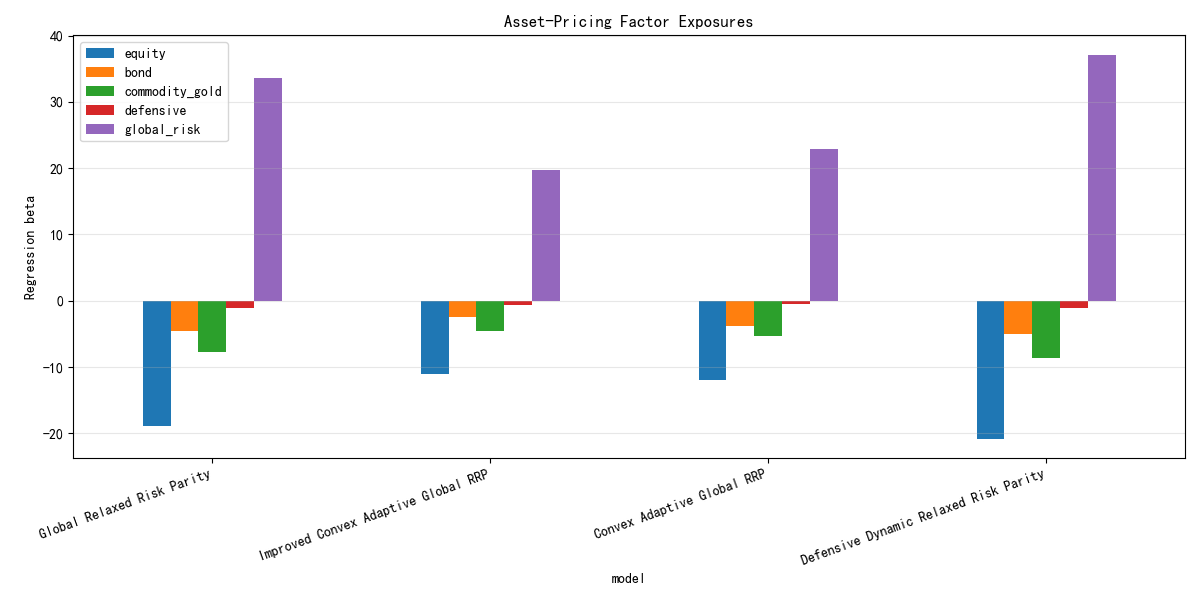
\includegraphics[width=0.88\textwidth]{asset_pricing_factor_exposure.png}
  \end{center}
\end{frame}

\begin{frame}{静态权重演进：标准 → 宽松 → 全球}
  \begin{columns}[T]
    \begin{column}{0.32\textwidth}
      \centering
      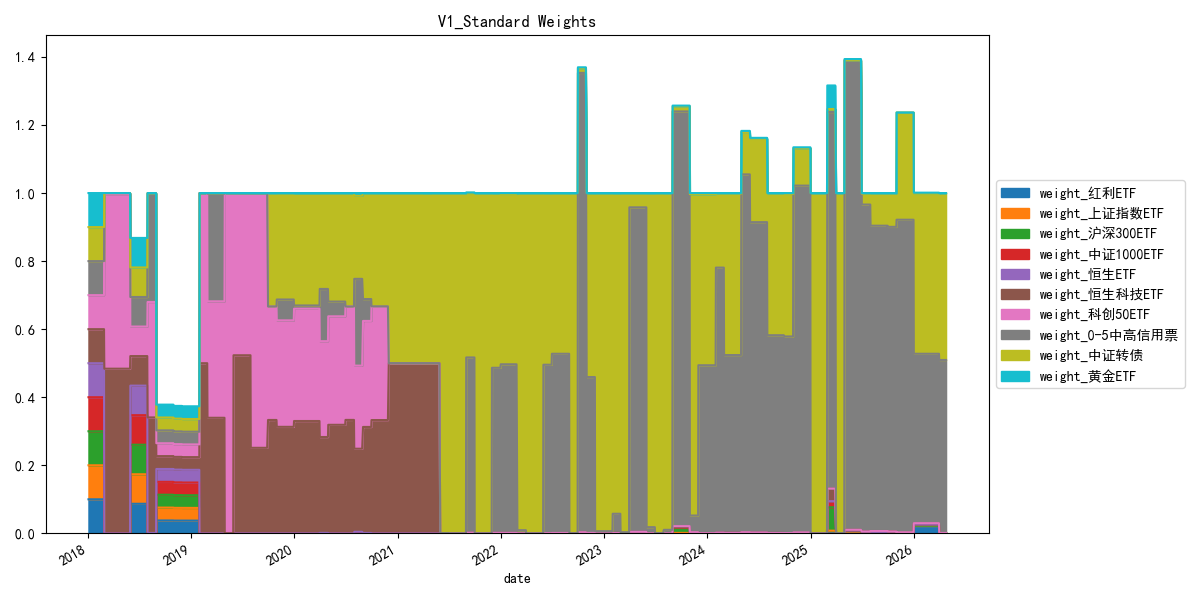
\includegraphics[width=\textwidth]{static_v1_standard_weights.png}\\
      \footnotesize 标准风险平价
    \end{column}
    \begin{column}{0.32\textwidth}
      \centering
      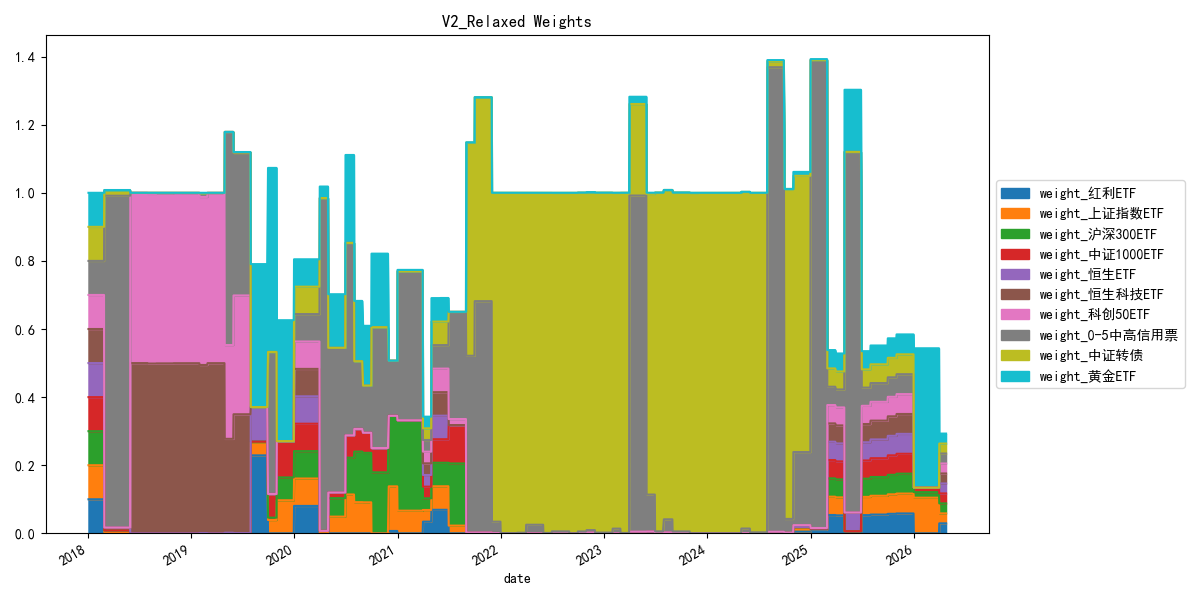
\includegraphics[width=\textwidth]{static_v2_relaxed_weights.png}\\
      \footnotesize 宽松 RRP
    \end{column}
    \begin{column}{0.32\textwidth}
      \centering
      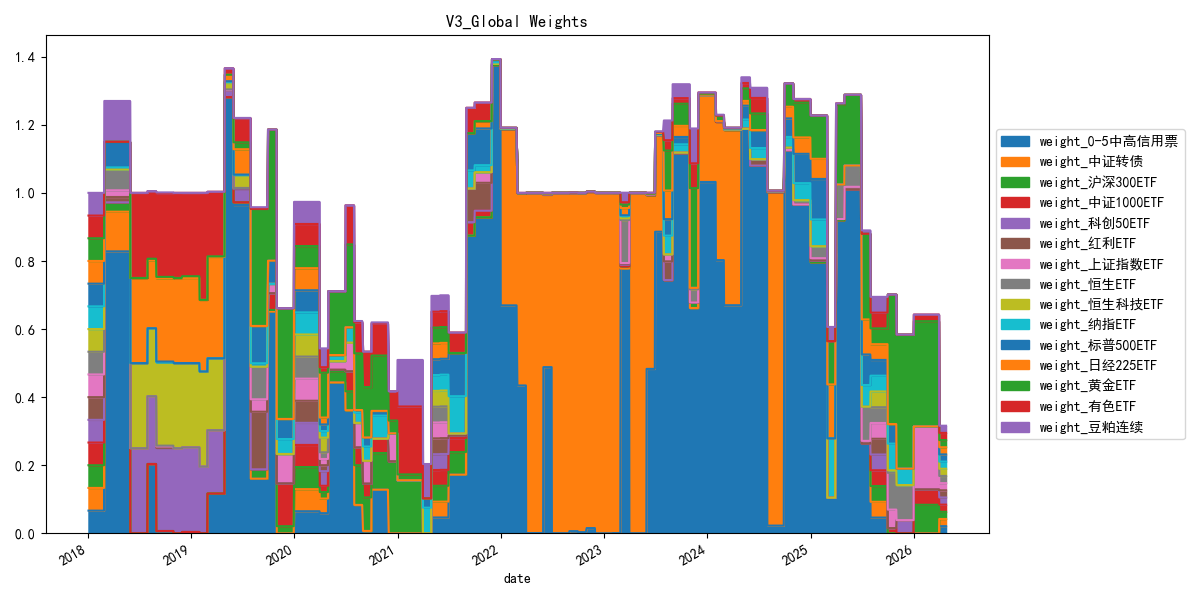
\includegraphics[width=\textwidth]{static_v3_global_weights.png}\\
      \footnotesize Global RRP（30 支）
    \end{column}
  \end{columns}
\end{frame}

% ════════════════════════════════════════════════════════════════════════════
\section{实证结果与分析}
% ════════════════════════════════════════════════════════════════════════════

\begin{frame}{绩效汇总（\evalStartDate{}—\evalEndDate{}）}
  \footnotesize
  \renewcommand{\arraystretch}{1.3}
  \begin{center}
    \begin{tabular}{@{}lcccccc@{}}
      \toprule
      模型 & 净年化收益 & Sharpe & Sortino & 最大回撤 & 月均换手 \\
      \midrule
      Global RRP        & \globalNetReturn  & \globalSharpe  & 0.770 & \globalMaxDD  & \globalMonthlyTurnover \\
      Convex Adaptive   & \convexNetReturn  & \convexSharpe  & 1.468 & \convexMaxDD  & \convexMonthlyTurnover \\
      \rowcolor{swufeLight}
      \textbf{Improved Convex} & \textbf{\improvedNetReturn} & \textbf{\improvedSharpe} & \textbf{\improvedSortino} & \textbf{\improvedMaxDD} & \textbf{\improvedMonthlyTurnover} \\
      HERC              & \hercNetReturn    & \hercSharpe    & 1.053 & \hercMaxDD    & 5.78\% \\
      \midrule
      等权基准 & \equalWeightNetReturn & \equalWeightSharpe & 1.276 & \equalWeightMaxDD & 1.24\% \\
      60/40 基准 & \sixtyFortyNetReturn & \sixtyFortySharpe & 1.119 & \sixtyFortyMaxDD & 1.43\% \\
      \bottomrule
    \end{tabular}
  \end{center}
  \scriptsize 无风险利率 \riskFreeRate{}；净收益已扣除 \txCostBps{} bps 单边成本
\end{frame}

\begin{frame}{净值路径：全模型对比}
  \begin{center}
    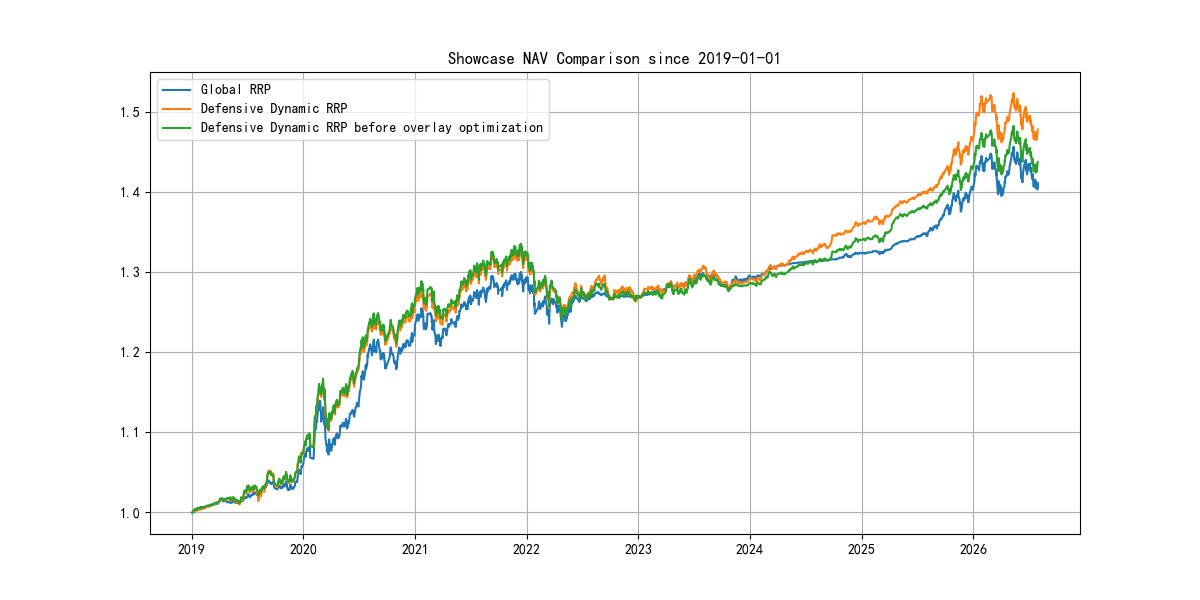
\includegraphics[width=0.90\textwidth]{showcase_nav_comparison.png}
  \end{center}
\end{frame}

\begin{frame}{回撤路径：全模型对比}
  \begin{center}
    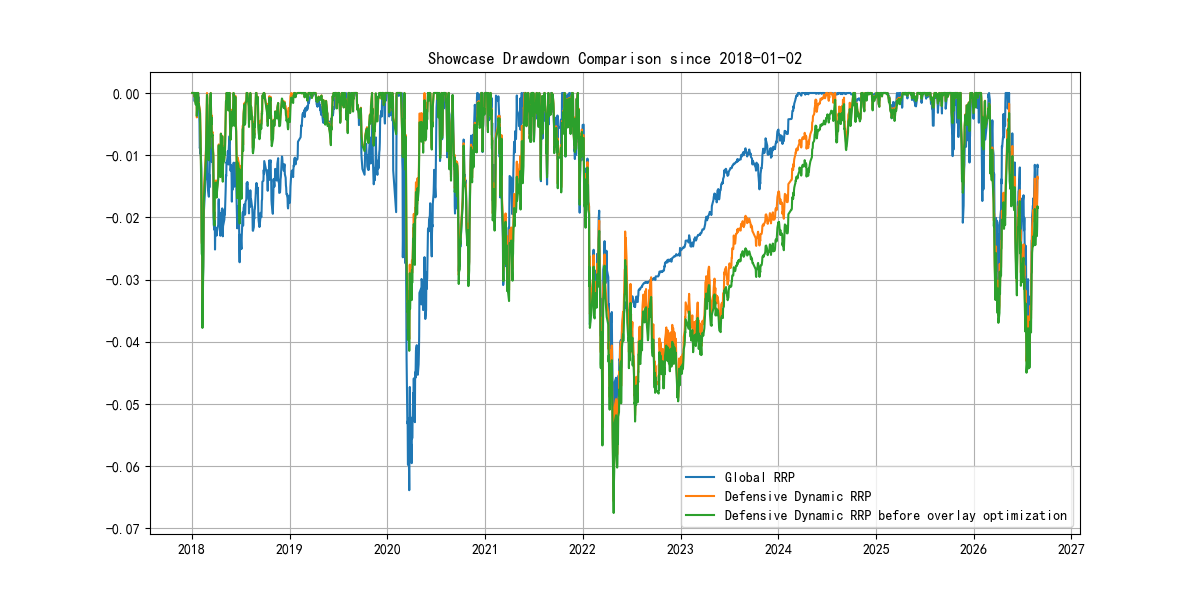
\includegraphics[width=0.90\textwidth]{showcase_drawdown_comparison.png}
  \end{center}
\end{frame}

\begin{frame}{静态基准 vs 动态模型：净值}
  \begin{center}
    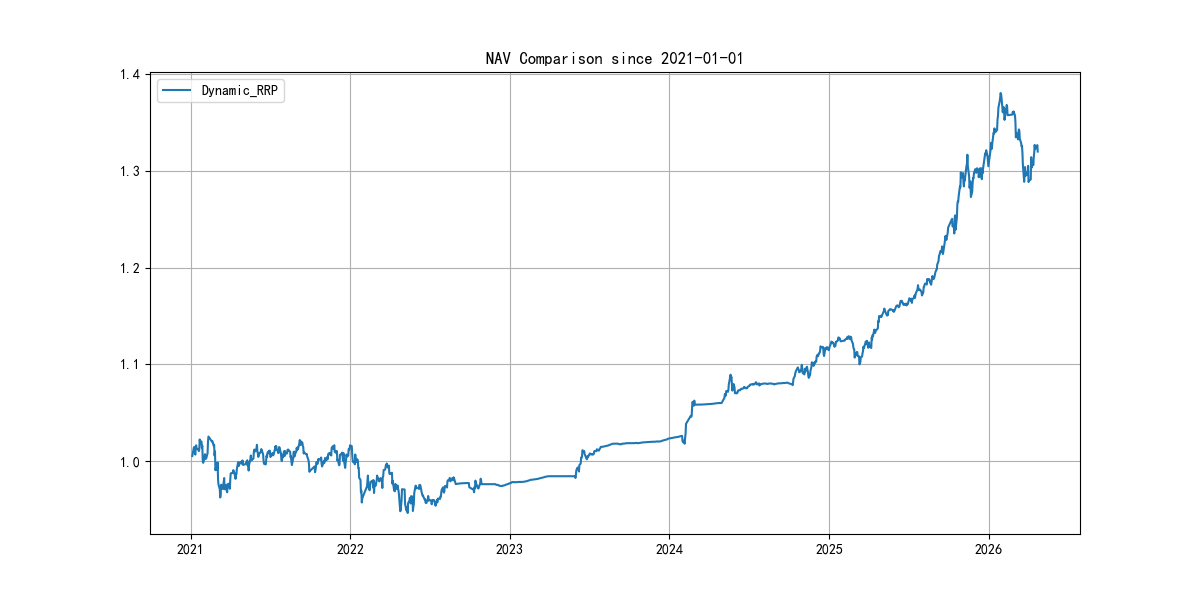
\includegraphics[width=0.90\textwidth]{static_vs_dynamic_nav.png}
  \end{center}
\end{frame}

\begin{frame}{Convex 系列净值对比}
  \begin{center}
    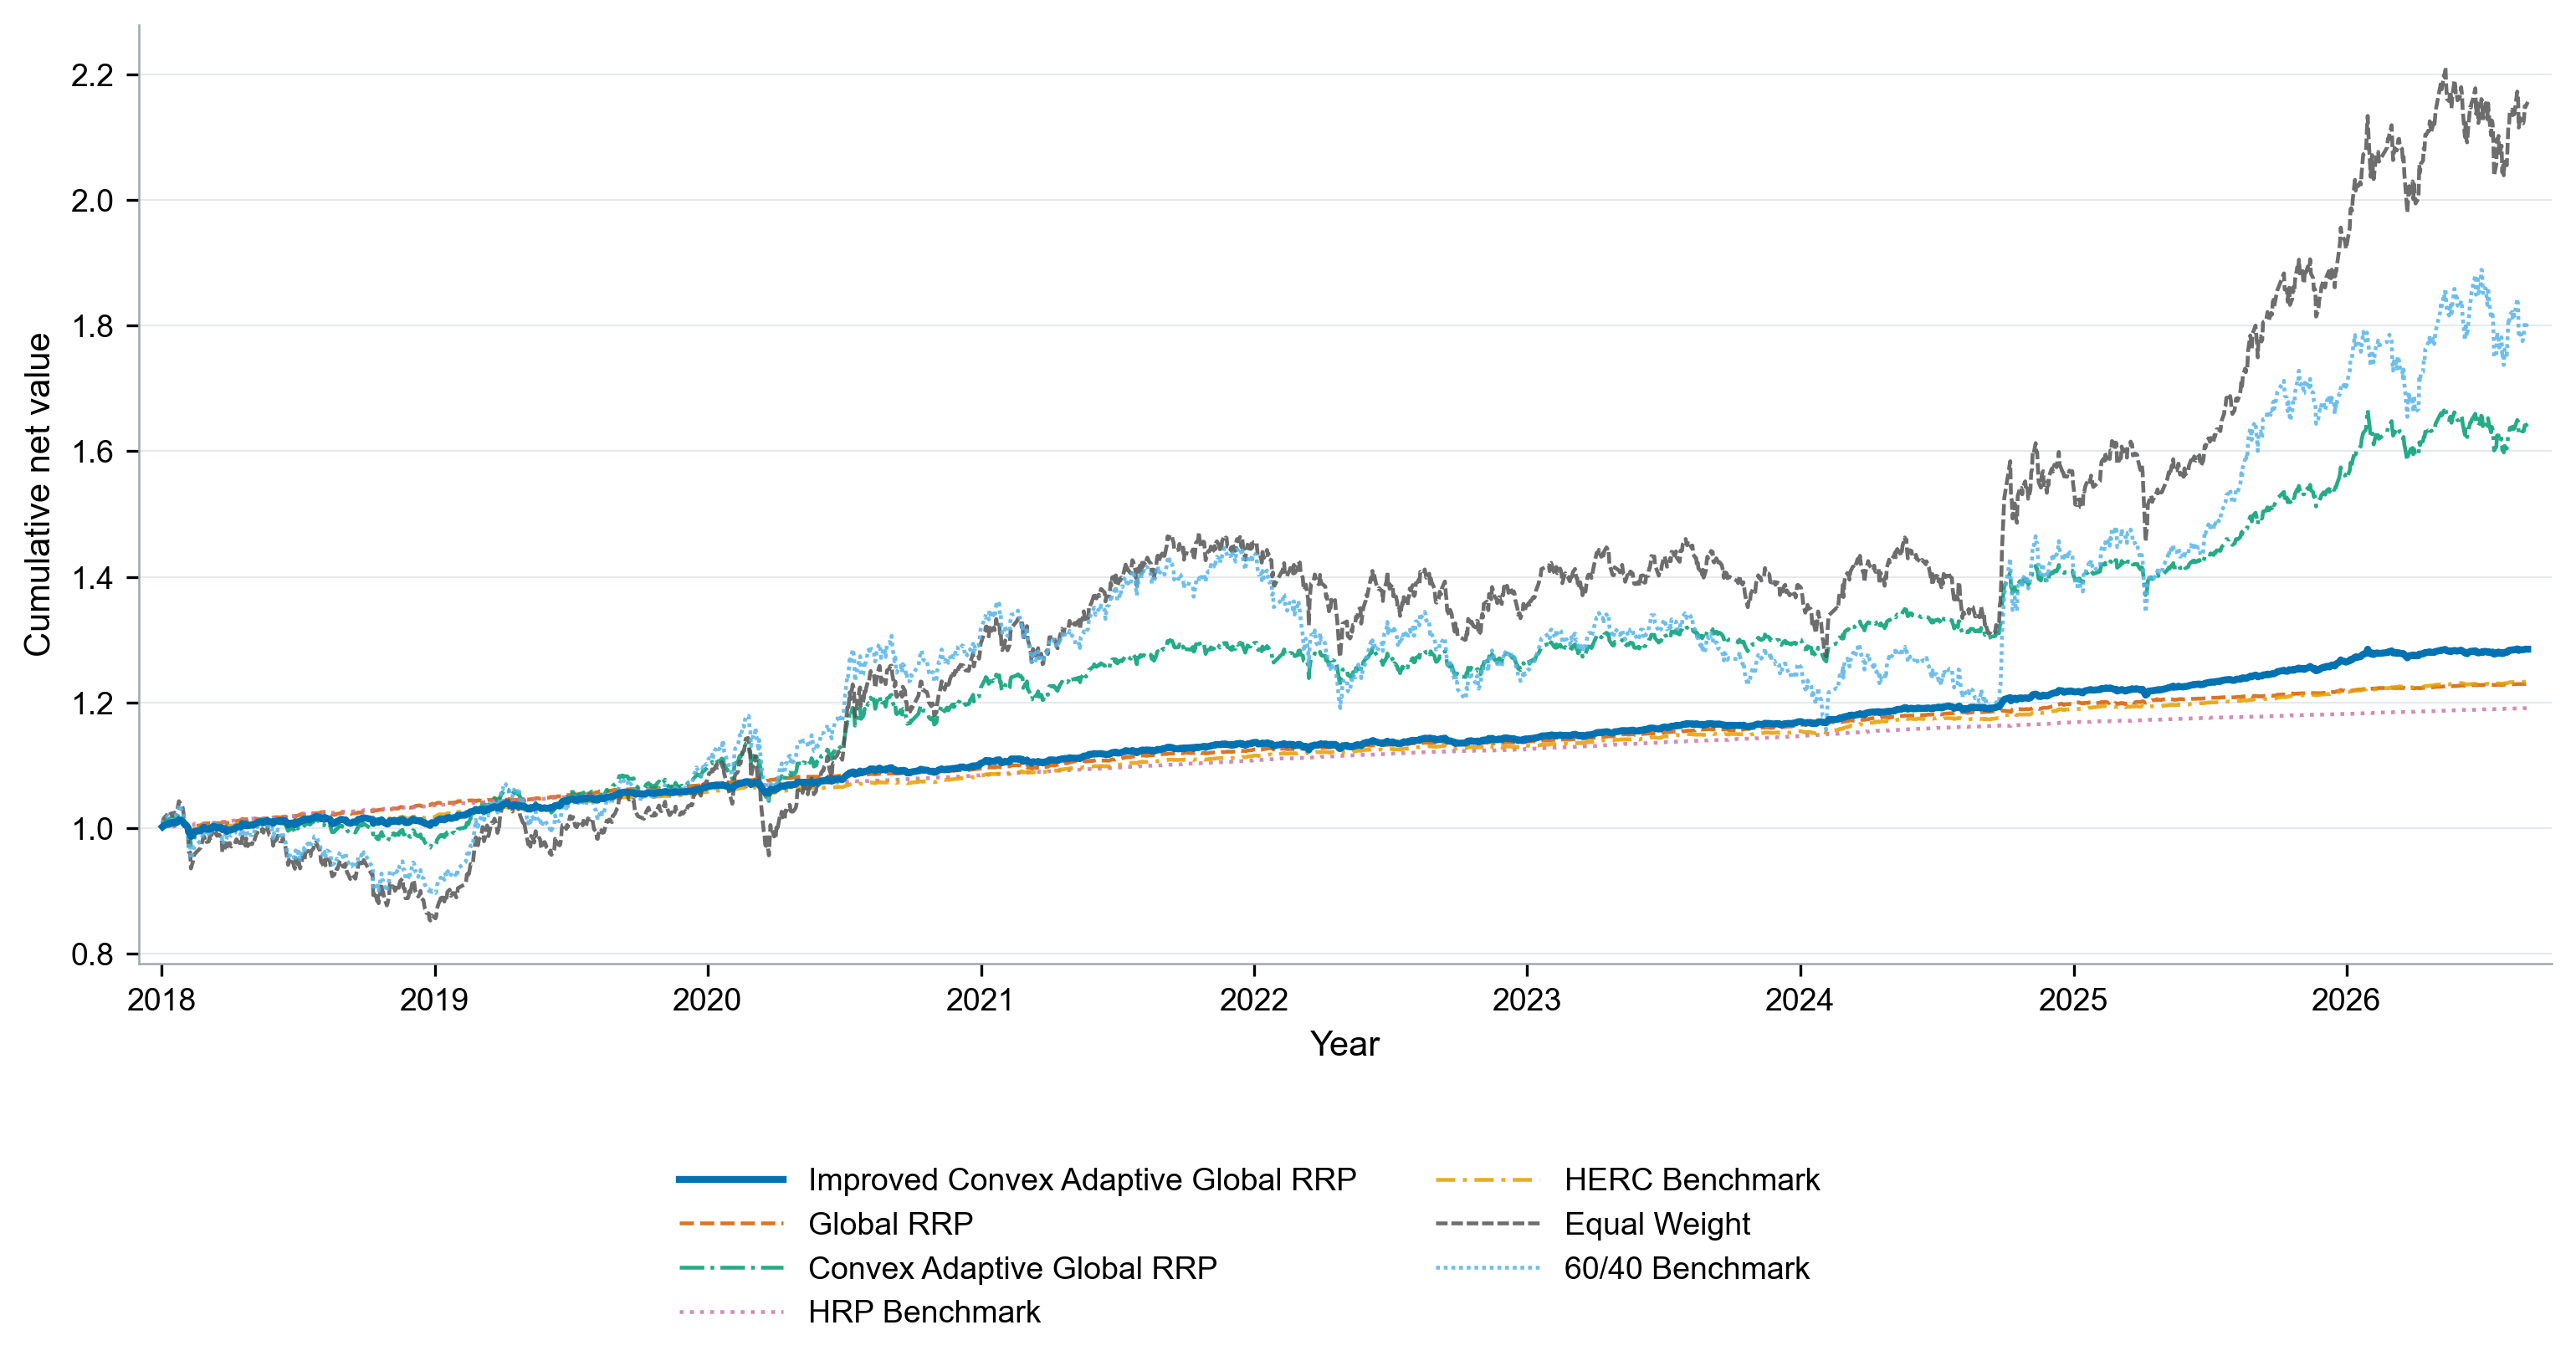
\includegraphics[width=0.90\textwidth]{convex_adaptive_nav_comparison.png}
  \end{center}
\end{frame}

\begin{frame}{Convex 系列回撤对比}
  \begin{center}
    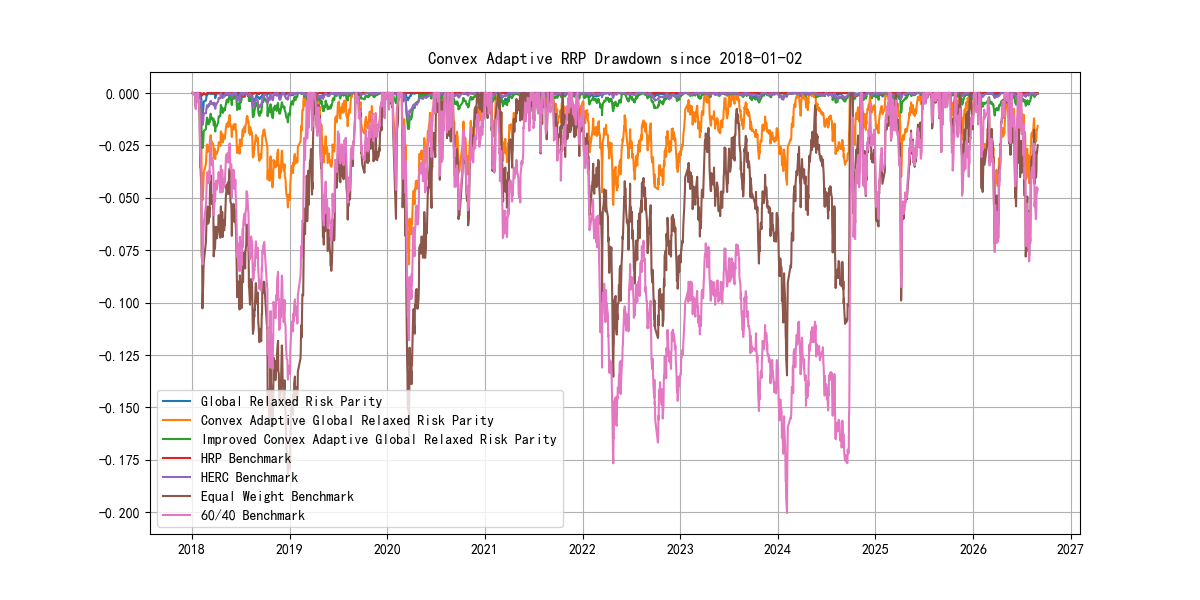
\includegraphics[width=0.90\textwidth]{convex_adaptive_drawdown_comparison.png}
  \end{center}
\end{frame}

\begin{frame}{换手率：CVaR + 惩罚项的效果}
  \begin{center}
    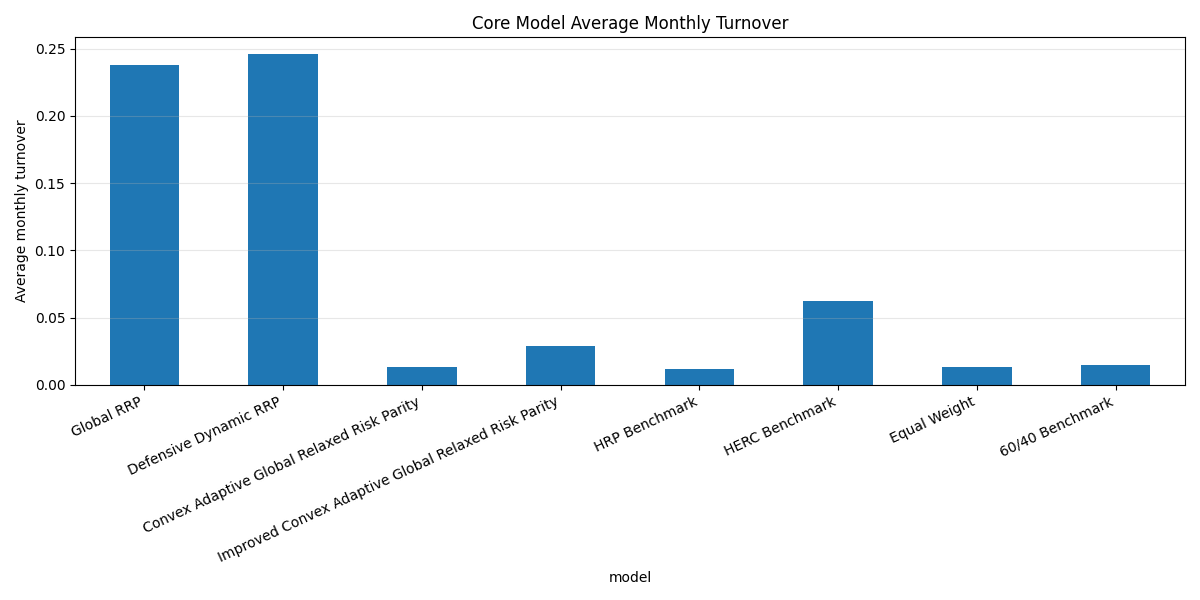
\includegraphics[width=0.90\textwidth]{convex_adaptive_turnover_comparison.png}
  \end{center}
  \begin{center}
    \footnotesize Global RRP 月均换手 \globalMonthlyTurnover{} → Improved Convex 压至 \textbf{\improvedMonthlyTurnover}（降低约 \textbf{10 倍}）
  \end{center}
\end{frame}

\begin{frame}{交易成本拖累对比}
  \begin{center}
    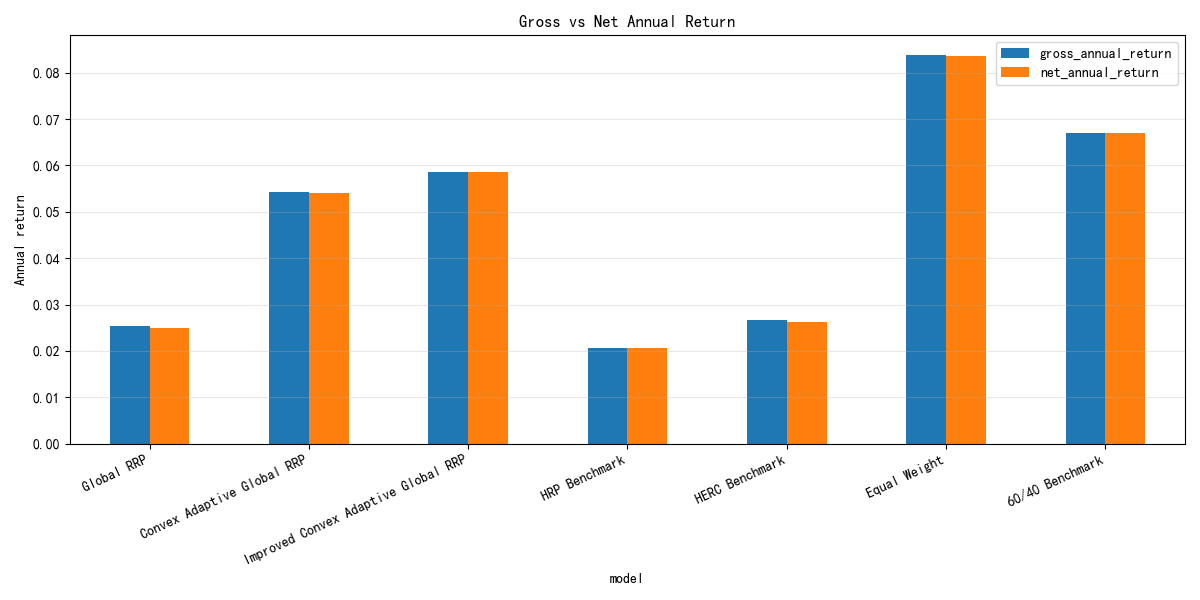
\includegraphics[width=0.90\textwidth]{convex_adaptive_transaction_cost_comparison.png}
  \end{center}
\end{frame}

\begin{frame}{CVaR 对比}
  \begin{center}
    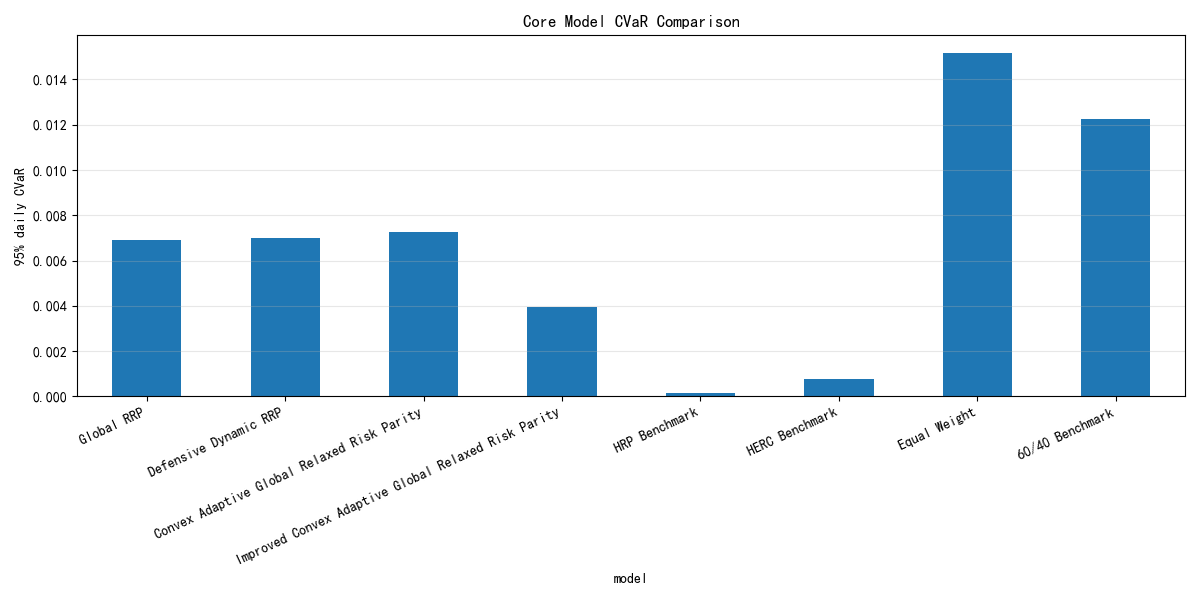
\includegraphics[width=0.90\textwidth]{convex_adaptive_cvar_comparison.png}
  \end{center}
\end{frame}

\begin{frame}{Improved Convex：权重动态路径}
  \begin{center}
    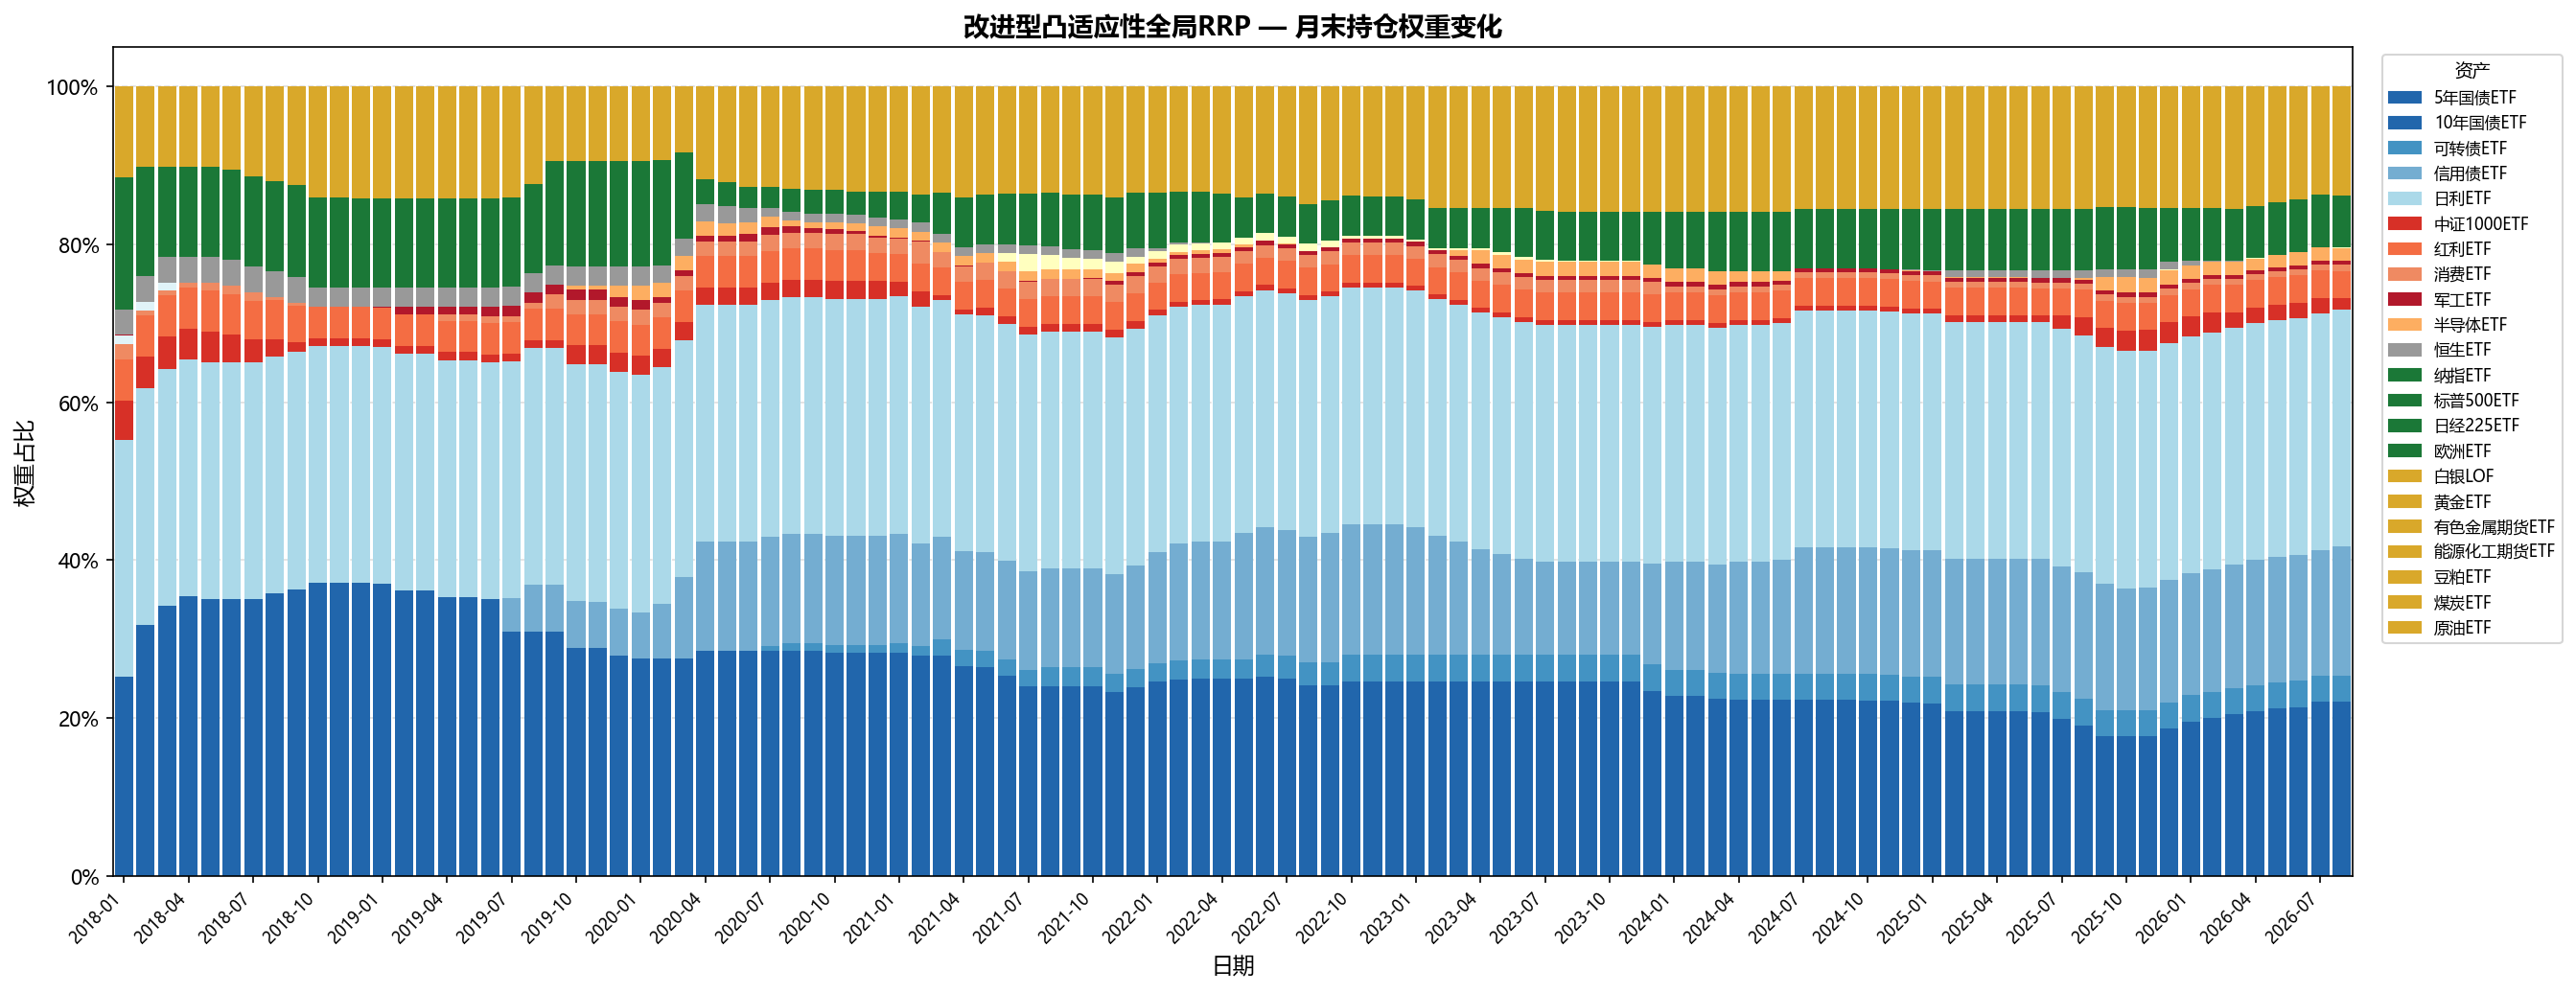
\includegraphics[width=0.90\textwidth]{improved_weights_timeline.png}
  \end{center}
\end{frame}

\begin{frame}{资产组权重路径对比}
  \begin{center}
    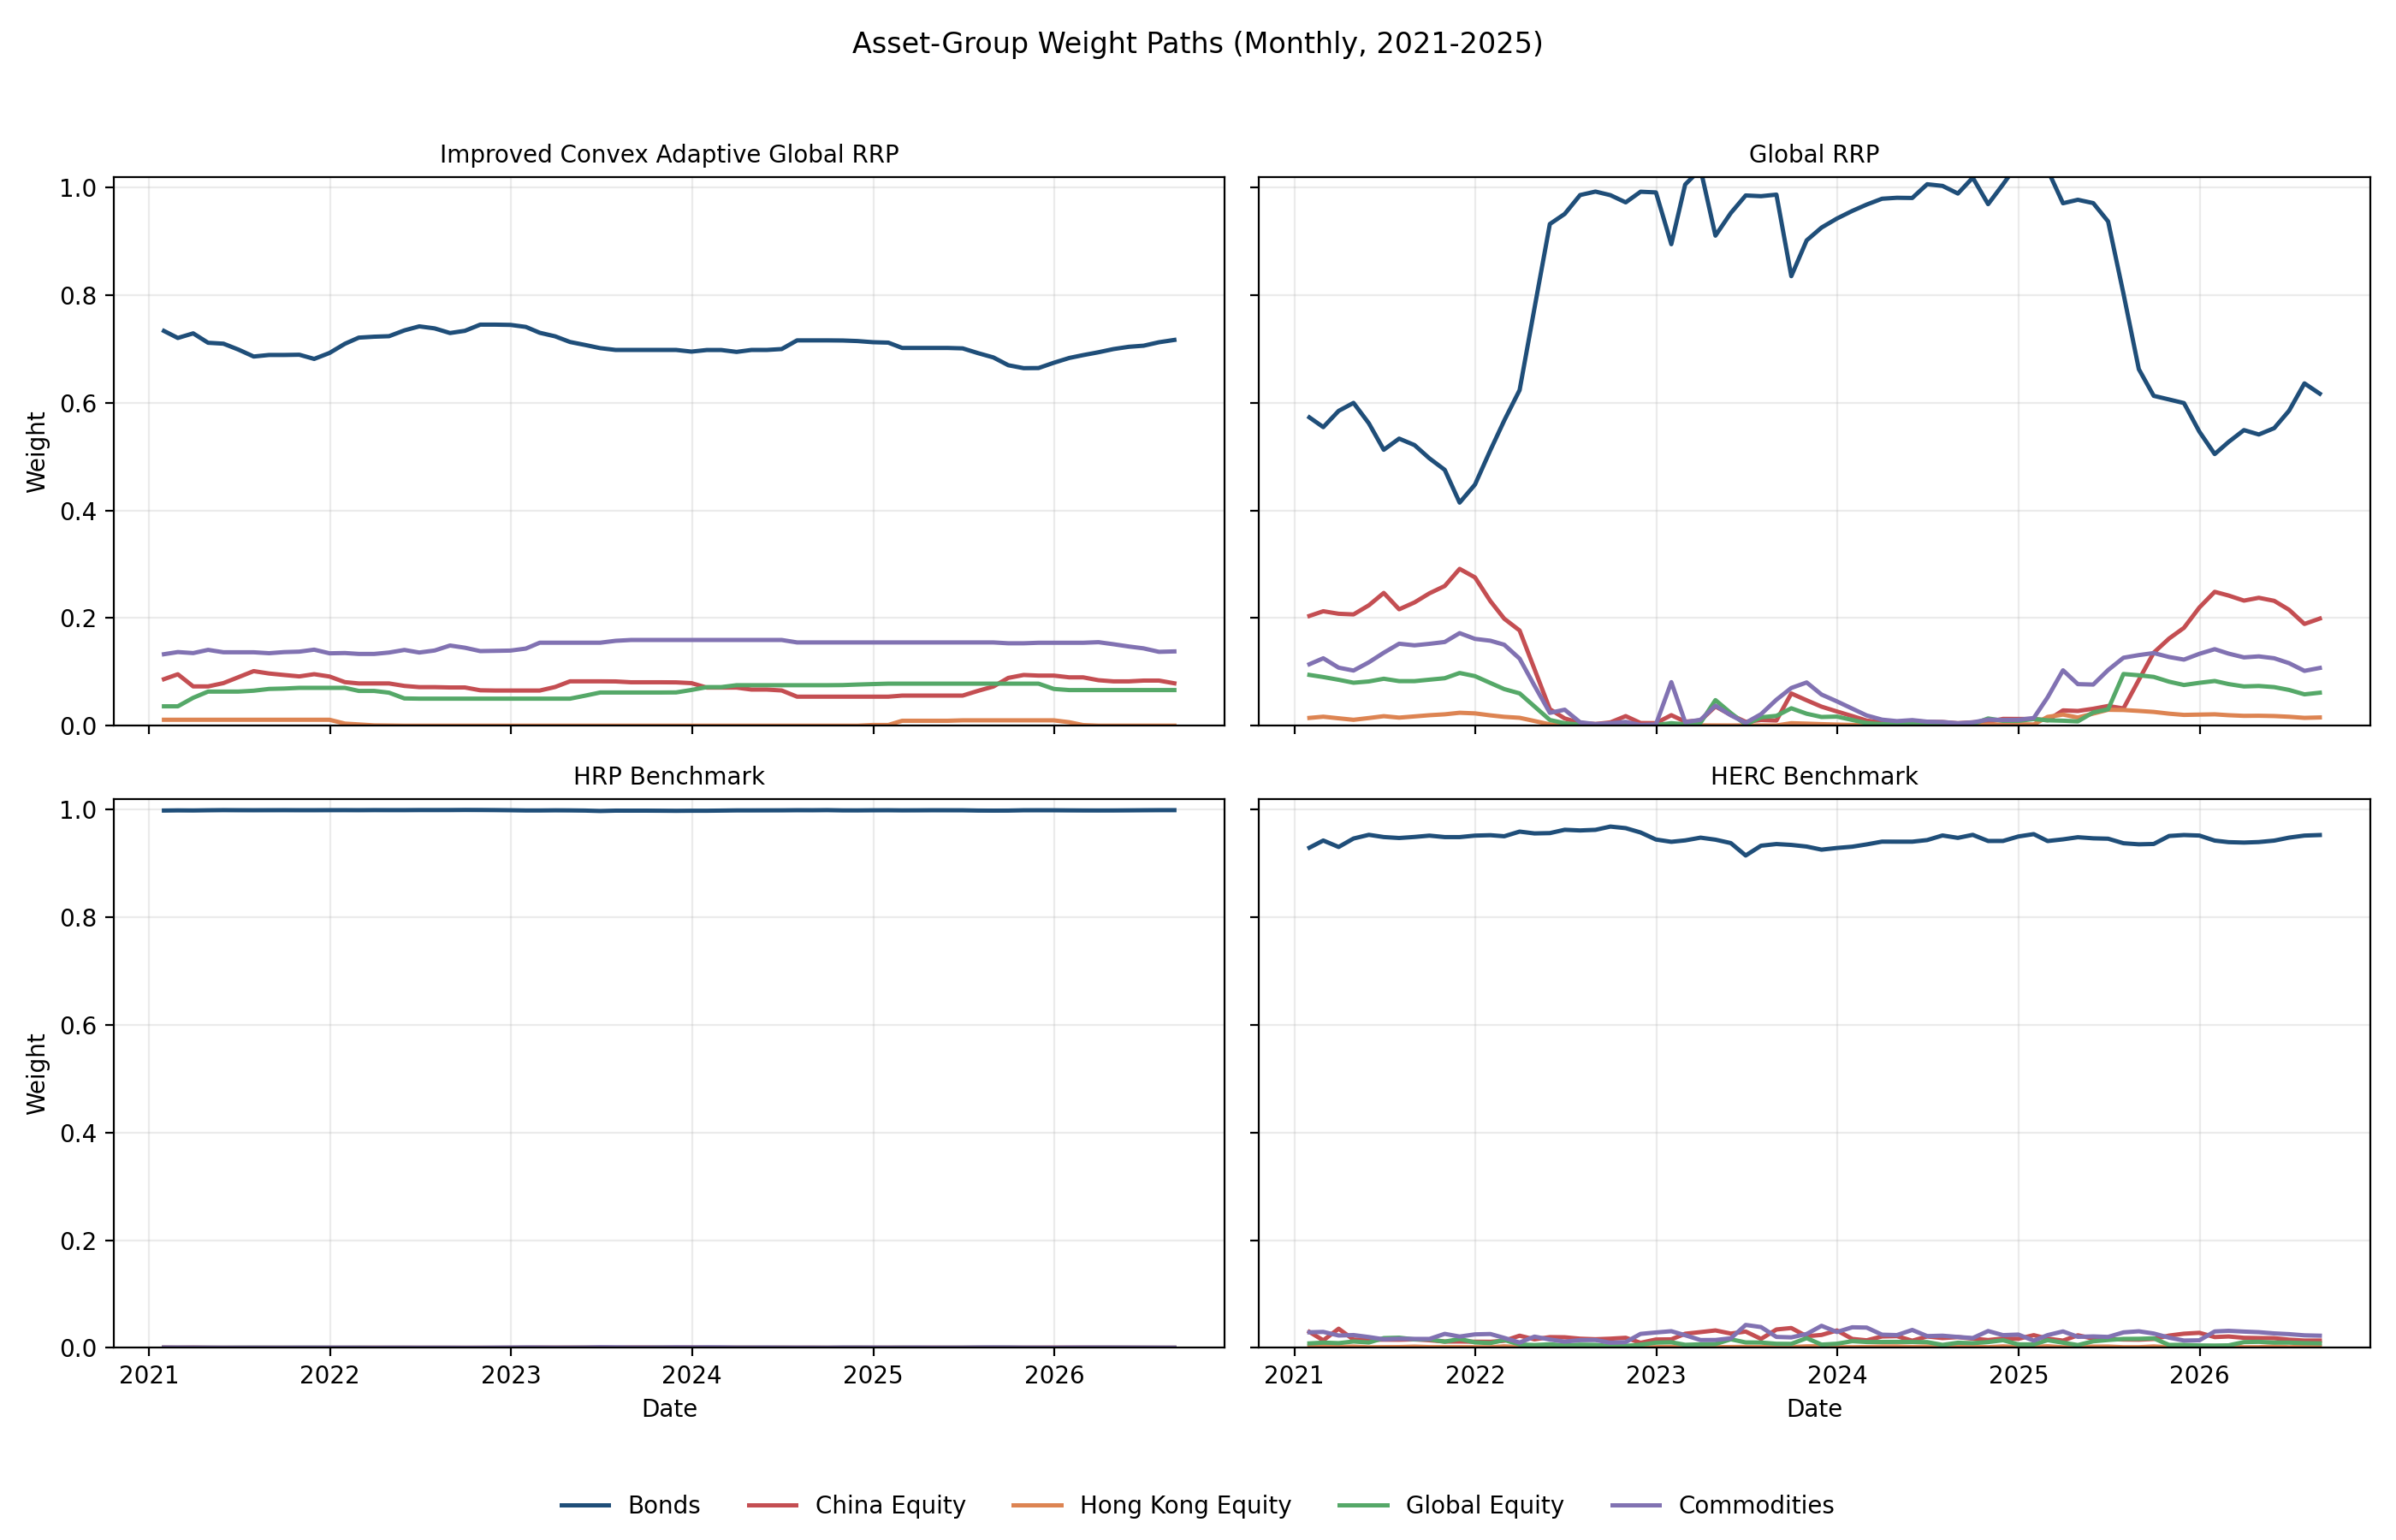
\includegraphics[width=0.90\textwidth]{weight_path_asset_group_comparison.png}
  \end{center}
\end{frame}

\begin{frame}{HERC 权重路径（为何 Sharpe 高但无可比性）}
  \begin{center}
    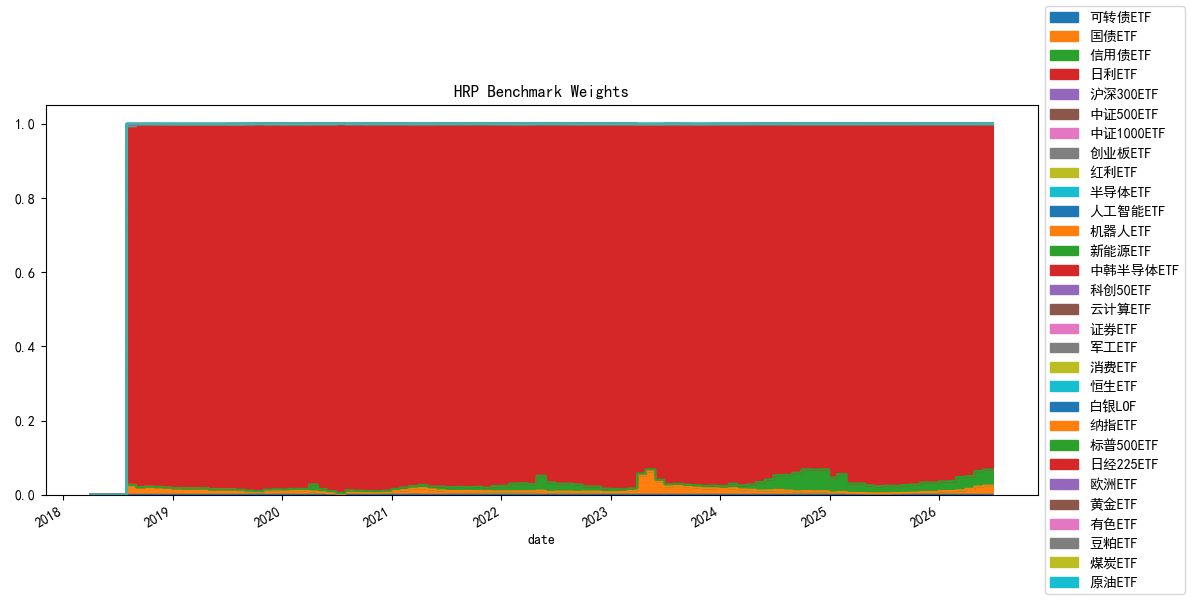
\includegraphics[width=0.90\textwidth]{hrp_weights_timeline.png}
  \end{center}
  \begin{center}
    \footnotesize HERC 近乎全仓债券/货币市场，年化波动率仅 0.57\%，Sharpe 来自人工压低波动，非多资产分散
  \end{center}
\end{frame}

\begin{frame}{与外部基准对比：净值}
  \begin{center}
    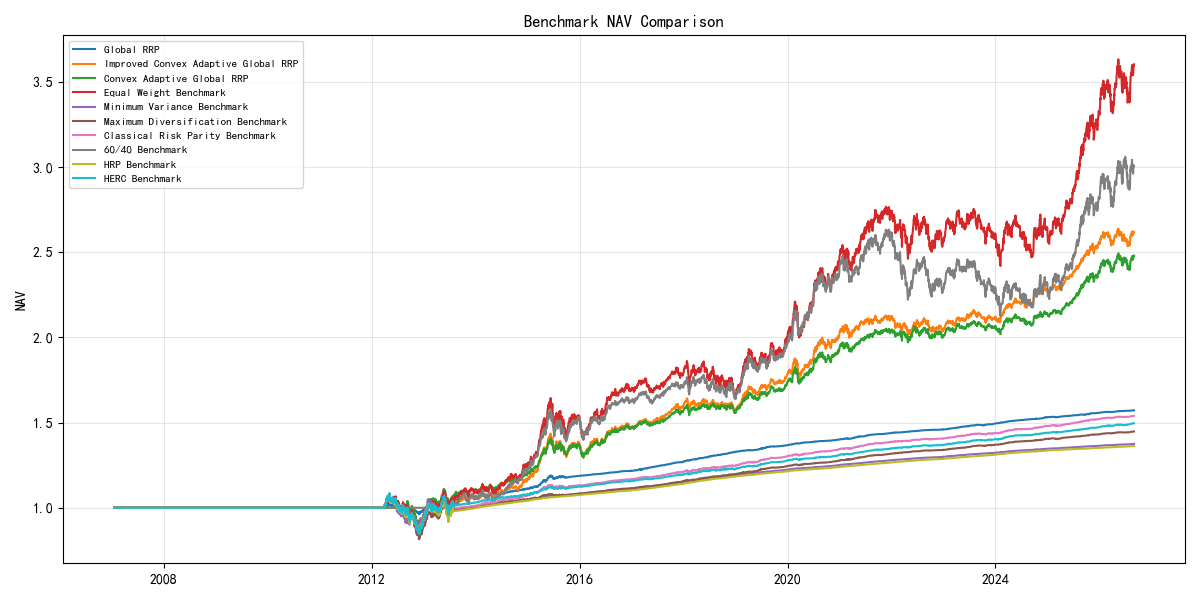
\includegraphics[width=0.90\textwidth]{benchmark_nav_comparison.png}
  \end{center}
\end{frame}

\begin{frame}{与外部基准对比：回撤}
  \begin{center}
    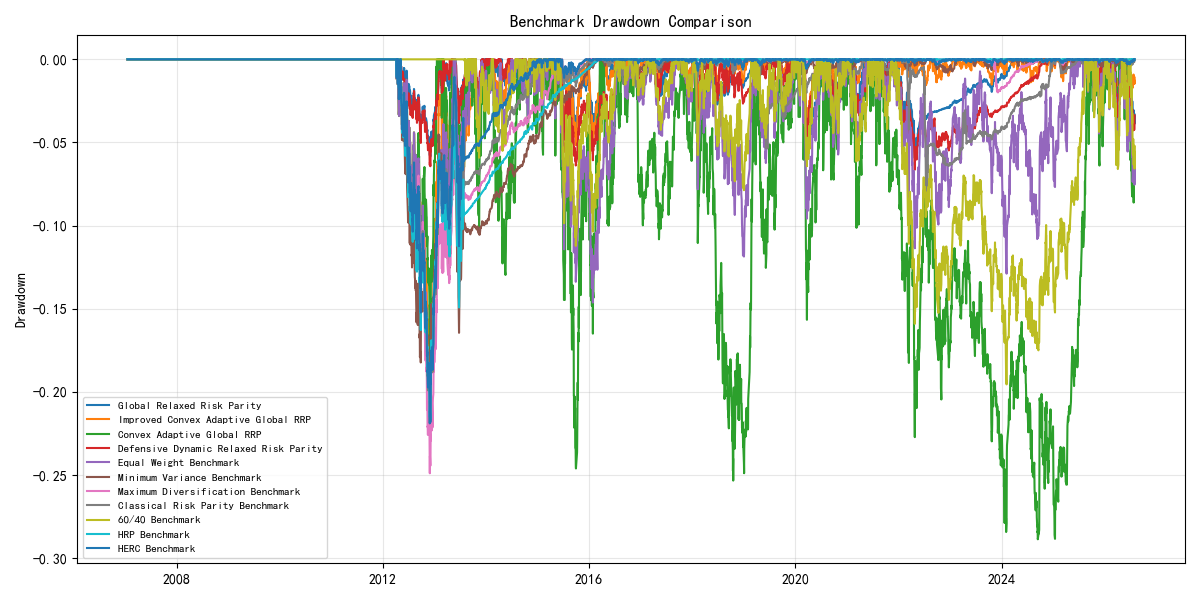
\includegraphics[width=0.90\textwidth]{benchmark_drawdown_comparison.png}
  \end{center}
\end{frame}

\begin{frame}{与沪深 300 月度收益对比}
  \begin{center}
    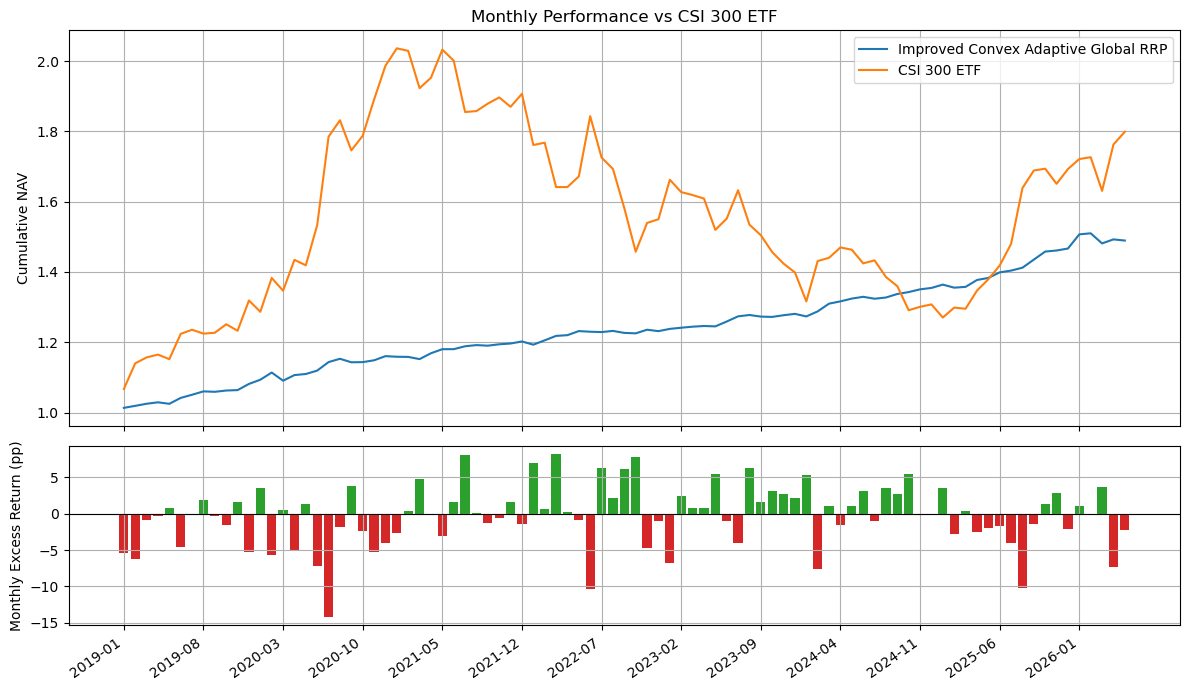
\includegraphics[width=0.90\textwidth]{improved_rrp_vs_hs300_monthly_comparison.png}
  \end{center}
\end{frame}

\begin{frame}{风险归因：各资产对组合波动的贡献}
  \begin{center}
    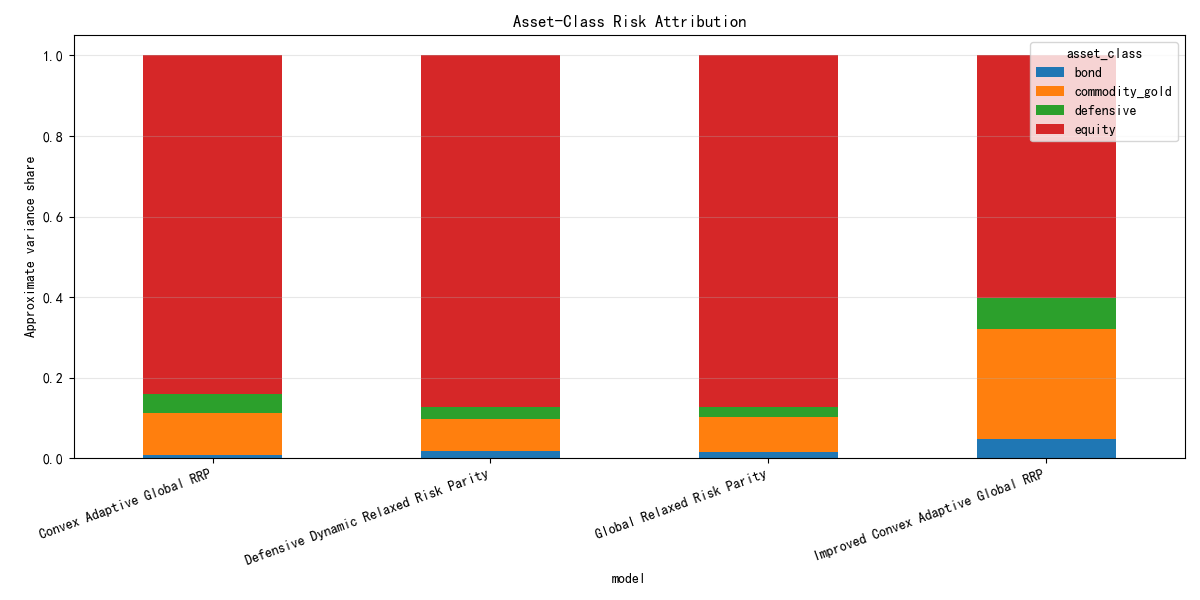
\includegraphics[width=0.90\textwidth]{asset_pricing_risk_attribution.png}
  \end{center}
\end{frame}

\begin{frame}{收益归因：各资产对组合净值的贡献}
  \begin{center}
    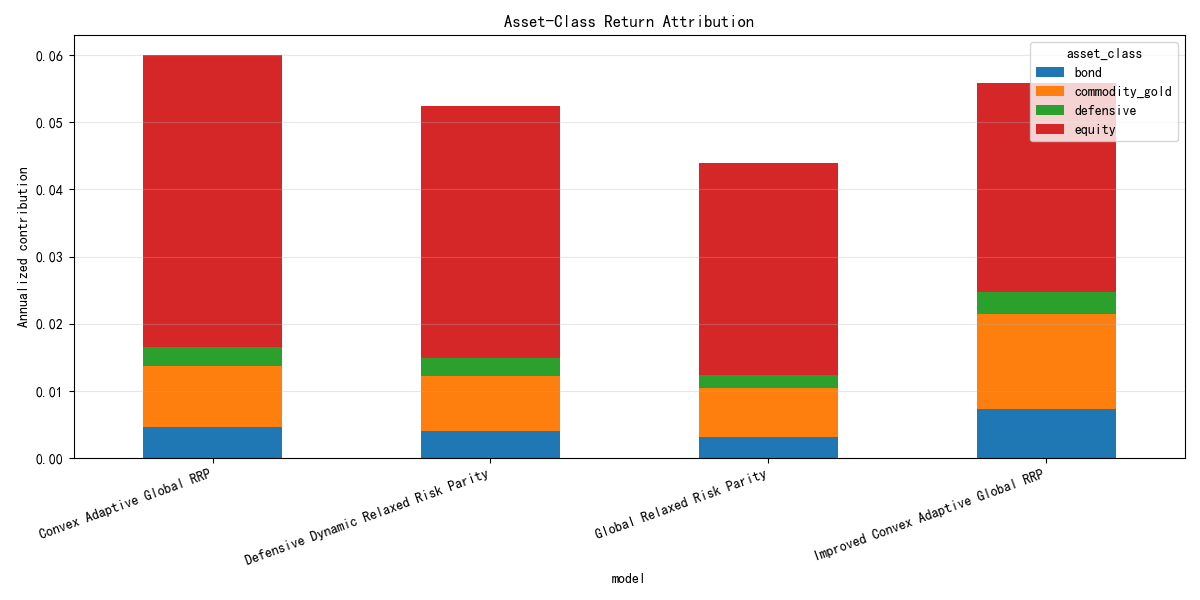
\includegraphics[width=0.90\textwidth]{asset_pricing_return_attribution.png}
  \end{center}
\end{frame}

\begin{frame}{滚动因子 Beta 时序}
  \begin{center}
    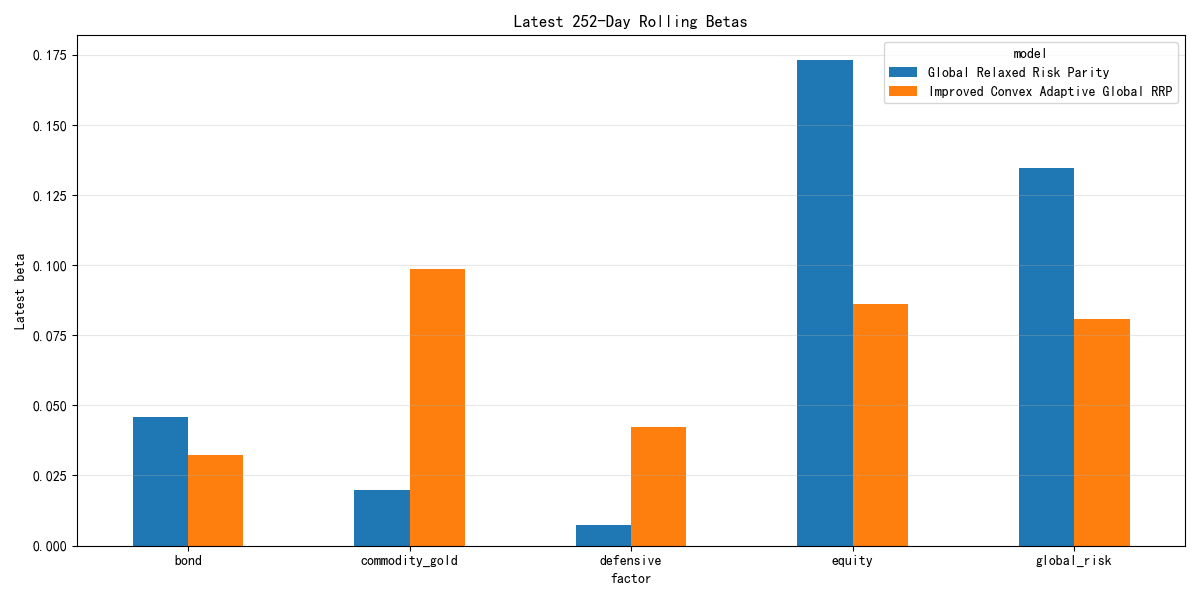
\includegraphics[width=0.90\textwidth]{asset_pricing_rolling_betas.png}
  \end{center}
\end{frame}

\begin{frame}{参数动态时序（$\lambda$ 选择）}
  \begin{center}
    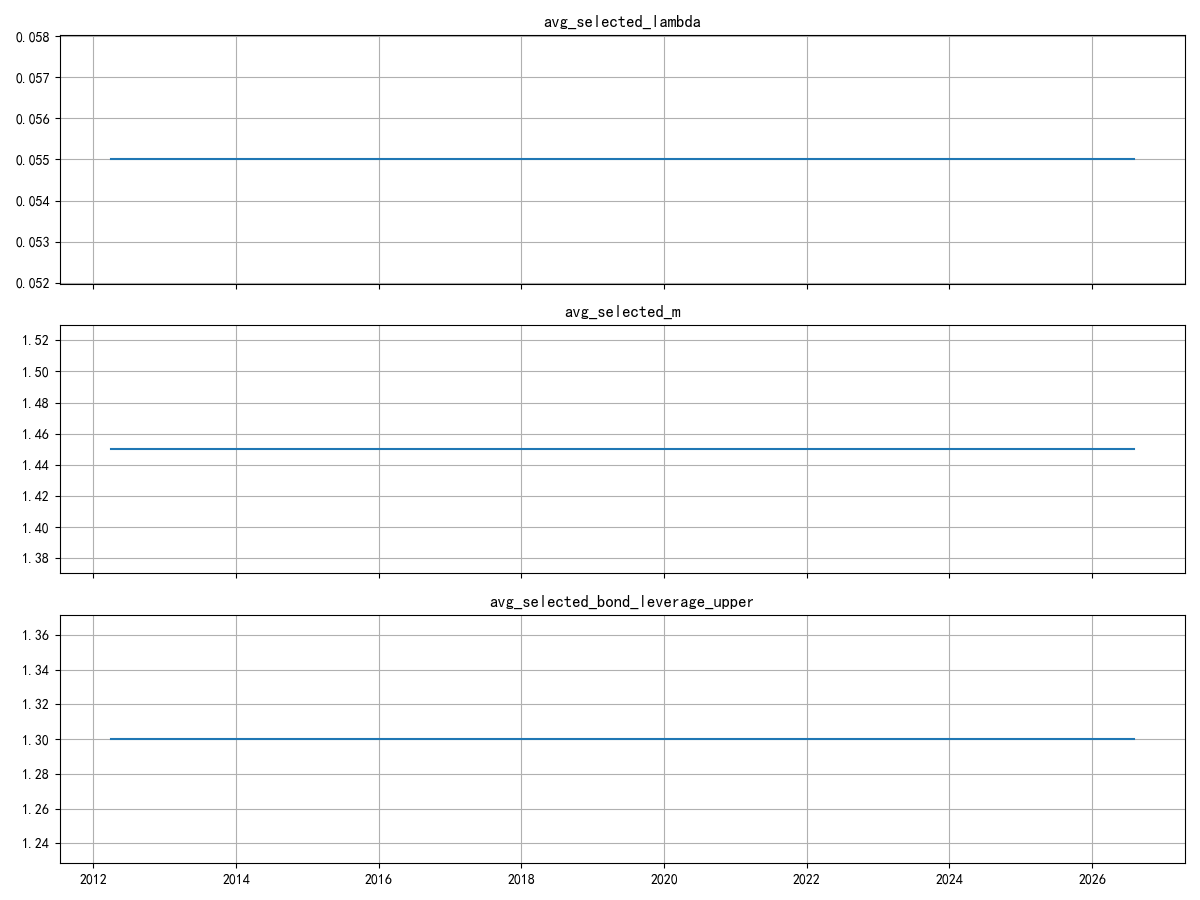
\includegraphics[width=0.90\textwidth]{showcase_parameter_timeline.png}
  \end{center}
\end{frame}

\begin{frame}{风险覆盖层消融实验}
  \begin{center}
    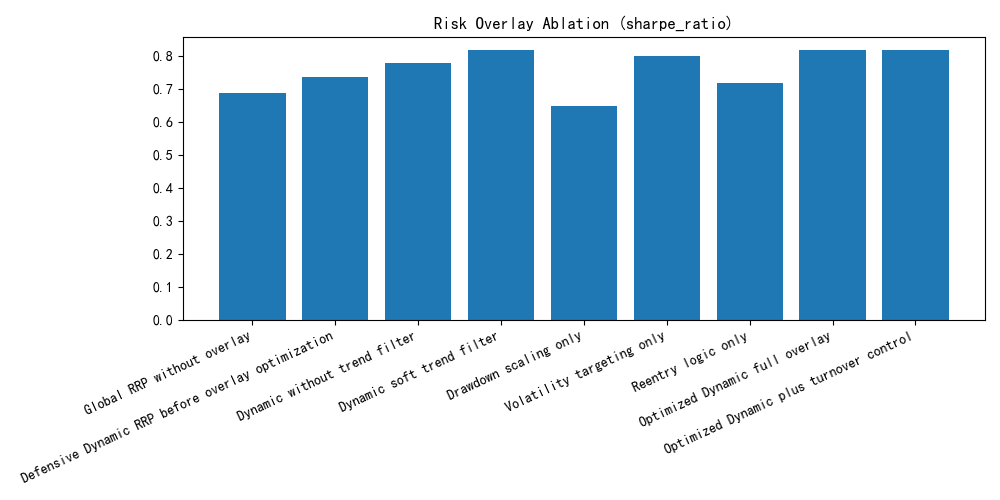
\includegraphics[width=0.90\textwidth]{showcase_risk_overlay_ablation.png}
  \end{center}
  \begin{center}
    \footnotesize 逐步剥离 CVaR 约束、换手惩罚和资产组上限，观察各约束对绩效的独立贡献
  \end{center}
\end{frame}

\begin{frame}{Sharpe 差异统计检验}
  \begin{columns}[T]
    \begin{column}{0.55\textwidth}
      \footnotesize
      \renewcommand{\arraystretch}{1.3}
      \begin{tabular}{@{}lccc@{}}
        \toprule
        比较对 & $\Delta$Sharpe & $p$ 值 & \\
        \midrule
        Improved vs.\ Global & \improvedVsGlobalDiff & \improvedVsGlobalPValue & \textbf{显著} \\
        Improved vs.\ Defensive & 0.893 & 0.001 & \textbf{显著} \\
        Improved vs.\ 等权 & 0.686 & 0.013 & \textbf{显著} \\
        Global vs.\ 等权 & $-$0.071 & 0.782 & 不显著 \\
        Defensive vs.\ 等权 & $-$0.185 & 0.434 & 不显著 \\
        \bottomrule
      \end{tabular}
      \vspace{0.3em}
      \scriptsize Jobson-Korkie 检验，Bootstrap 95\% CI
    \end{column}
    \begin{column}{0.42\textwidth}
      \begin{block}{核心含义}
        \small
        \begin{itemize}
          \item Improved Convex 的 Sharpe 优势\textbf{统计显著}（$p=0.004$）
          \item 仅降低换手不足以产生显著提升
          \item CVaR 约束 + 参数冻结是真实来源
        \end{itemize}
      \end{block}
    \end{column}
  \end{columns}
\end{frame}

% ════════════════════════════════════════════════════════════════════════════
\section{稳健性检验}
% ════════════════════════════════════════════════════════════════════════════

\begin{frame}{Walk-forward 子区间 Sharpe}
  \begin{center}
    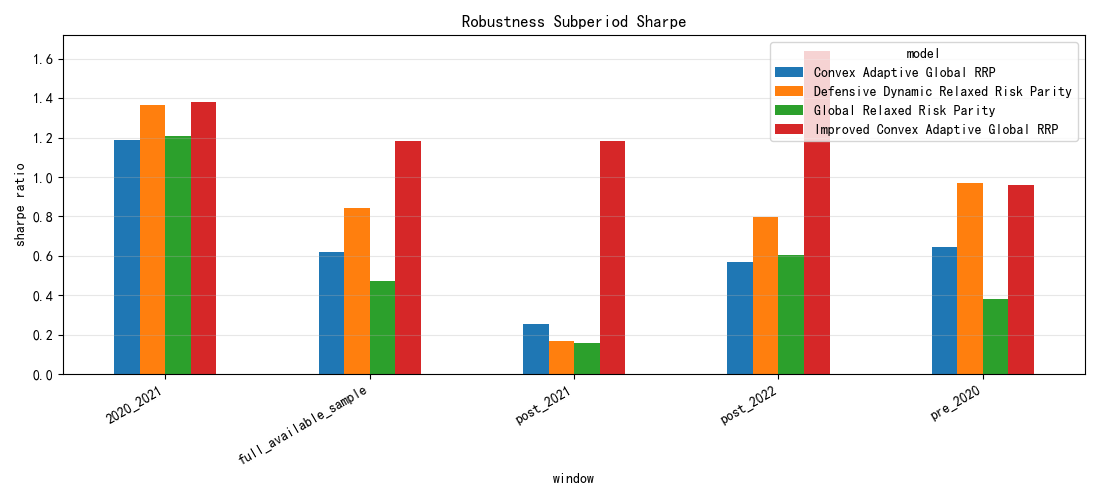
\includegraphics[width=0.90\textwidth]{robustness_subperiod_sharpe.png}
  \end{center}
  \begin{center}
    \footnotesize Walk-forward 中位数 Sharpe = \walkforwardSharpeMedian{}，均值 = \walkforwardSharpeMean{}，跨区间相对稳定
  \end{center}
\end{frame}

\begin{frame}{Walk-forward 子区间最大回撤}
  \begin{center}
    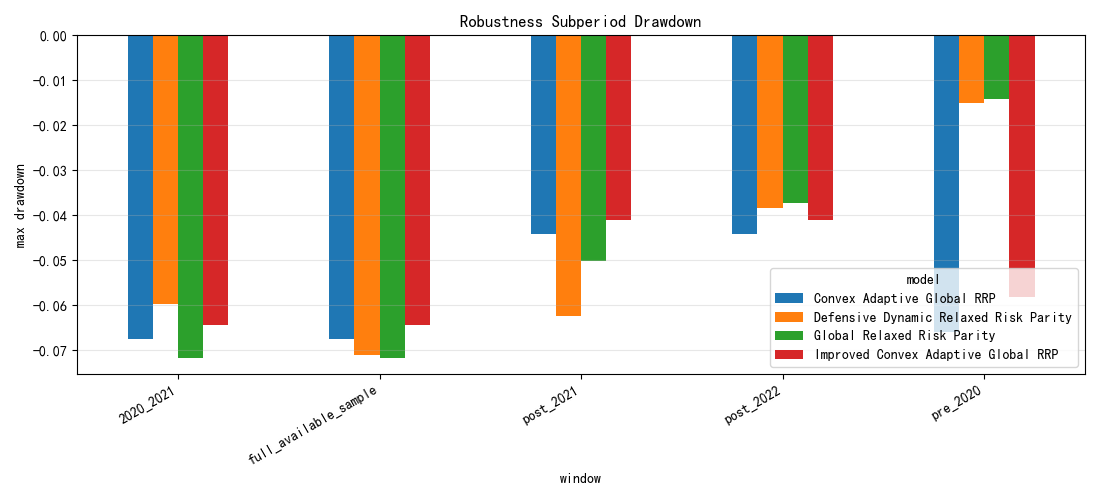
\includegraphics[width=0.90\textwidth]{robustness_subperiod_drawdown.png}
  \end{center}
\end{frame}

\begin{frame}{参数扰动敏感性分析}
  \begin{center}
    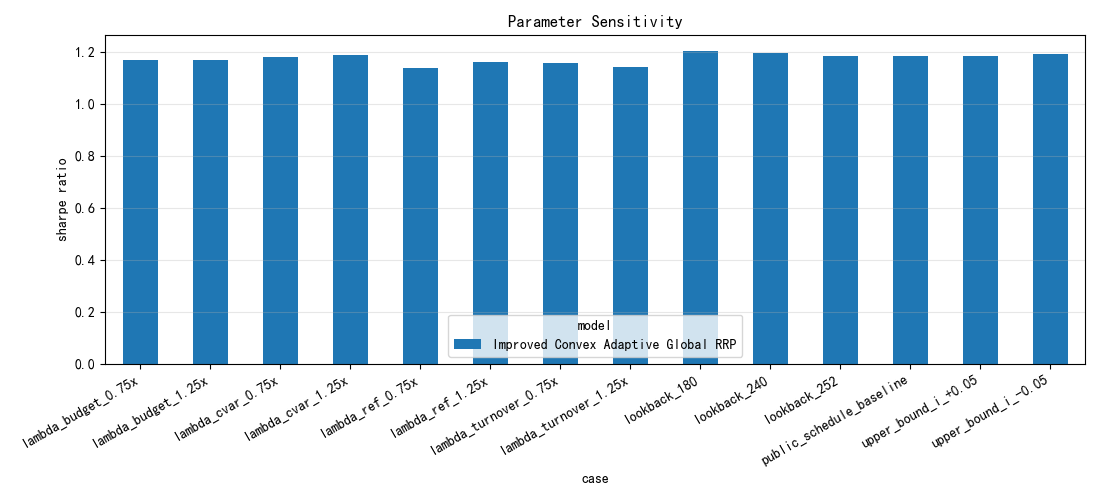
\includegraphics[width=0.90\textwidth]{robustness_parameter_sensitivity.png}
  \end{center}
\end{frame}

\begin{frame}{交易成本敏感性：盈亏平衡分析}
  \begin{center}
    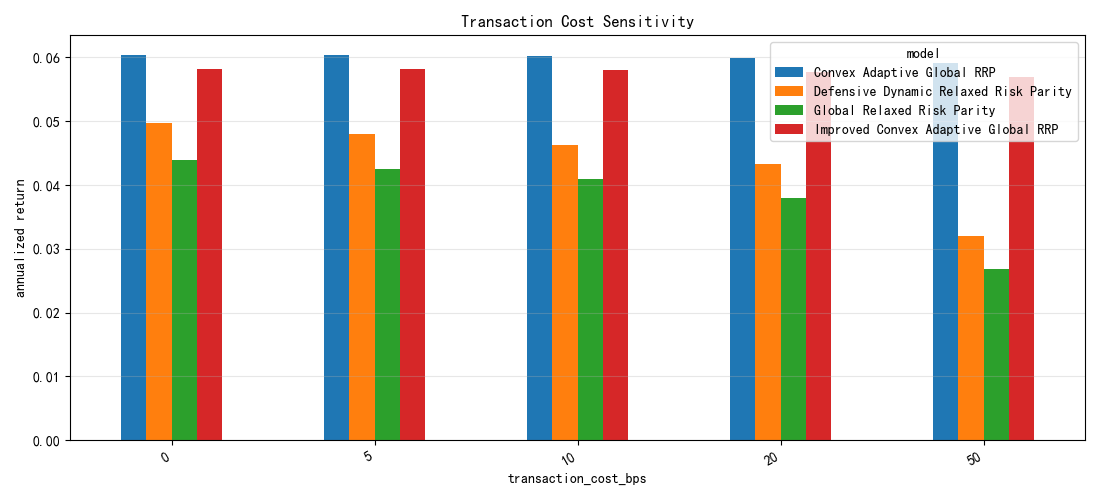
\includegraphics[width=0.90\textwidth]{robustness_transaction_cost_sensitivity.png}
  \end{center}
  \begin{center}
    \footnotesize Improved vs.\ Global RRP 盈亏平衡成本 $>$50 bps；实际 \txCostBps{} bps 远低于此阈值
  \end{center}
\end{frame}

\begin{frame}{Bootstrap Sharpe 分布}
  \begin{center}
    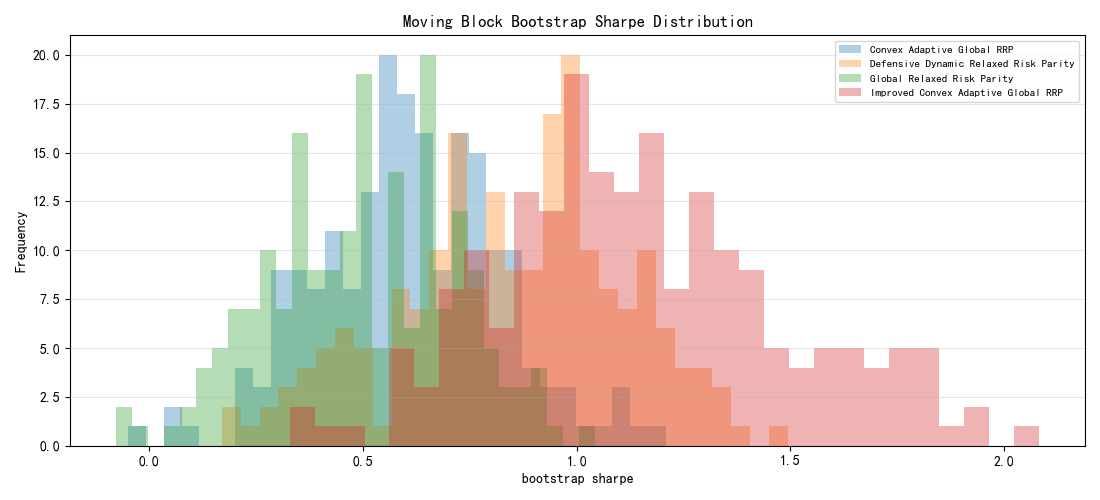
\includegraphics[width=0.90\textwidth]{robustness_bootstrap_sharpe_distribution.png}
  \end{center}
\end{frame}

\begin{frame}{Bootstrap 最大回撤分布}
  \begin{center}
    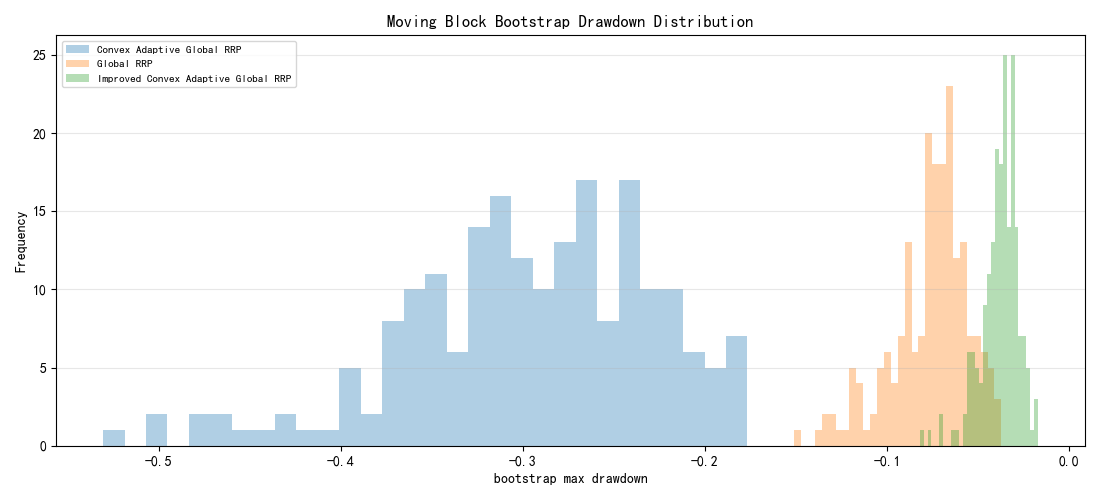
\includegraphics[width=0.90\textwidth]{robustness_bootstrap_drawdown_distribution.png}
  \end{center}
\end{frame}

\begin{frame}{过拟合诊断}
  \begin{center}
    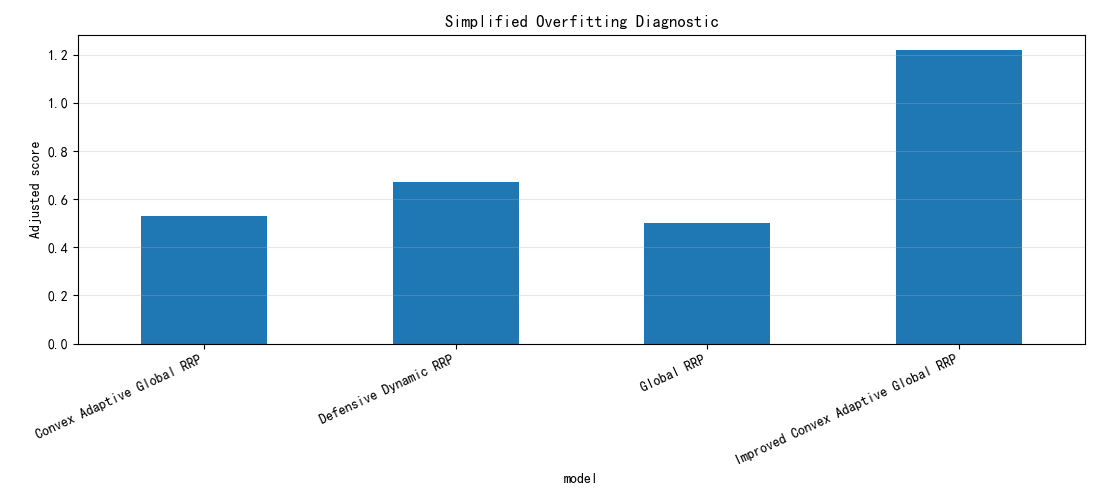
\includegraphics[width=0.90\textwidth]{robustness_overfitting_diagnostic.png}
  \end{center}
\end{frame}

\begin{frame}{PBO 热图（概率回测过拟合）}
  \begin{center}
    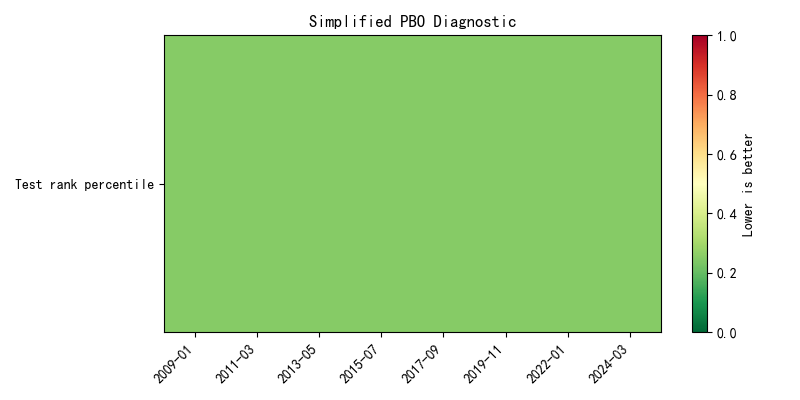
\includegraphics[width=0.90\textwidth]{showcase_pbo_heatmap.png}
  \end{center}
\end{frame}

\begin{frame}{协方差估计器对比：Sharpe 和换手}
  \begin{columns}[T]
    \begin{column}{0.50\textwidth}
      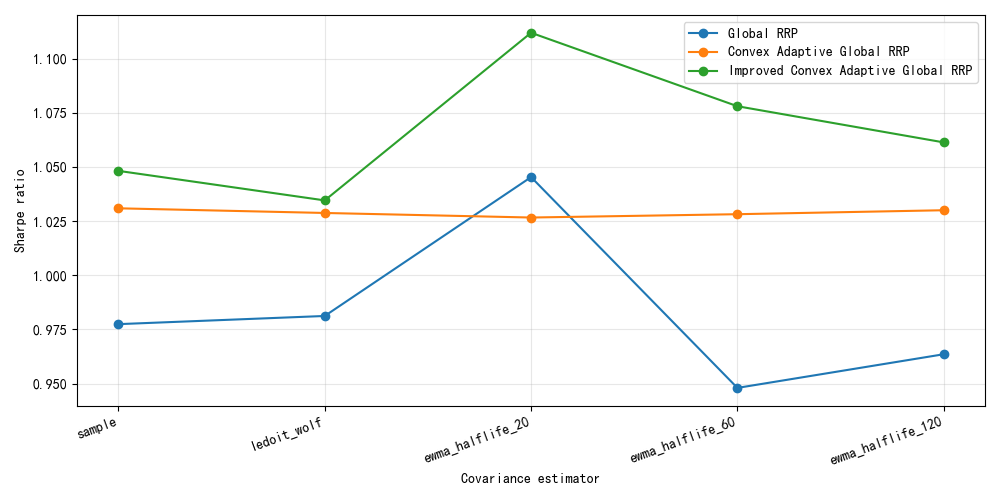
\includegraphics[width=\textwidth]{covariance_robustness_sharpe.png}
    \end{column}
    \begin{column}{0.50\textwidth}
      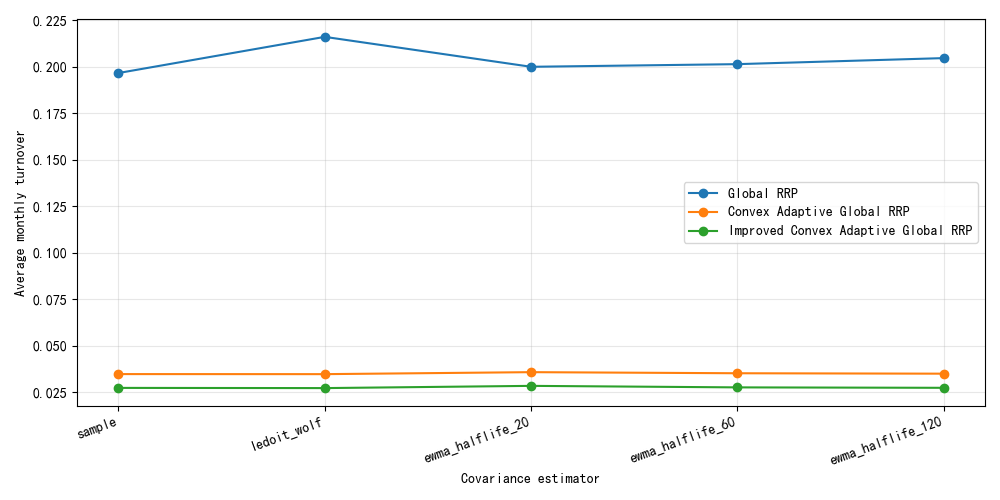
\includegraphics[width=\textwidth]{covariance_robustness_turnover.png}
    \end{column}
  \end{columns}
\end{frame}

\begin{frame}{协方差估计器对比：最大回撤}
  \begin{center}
    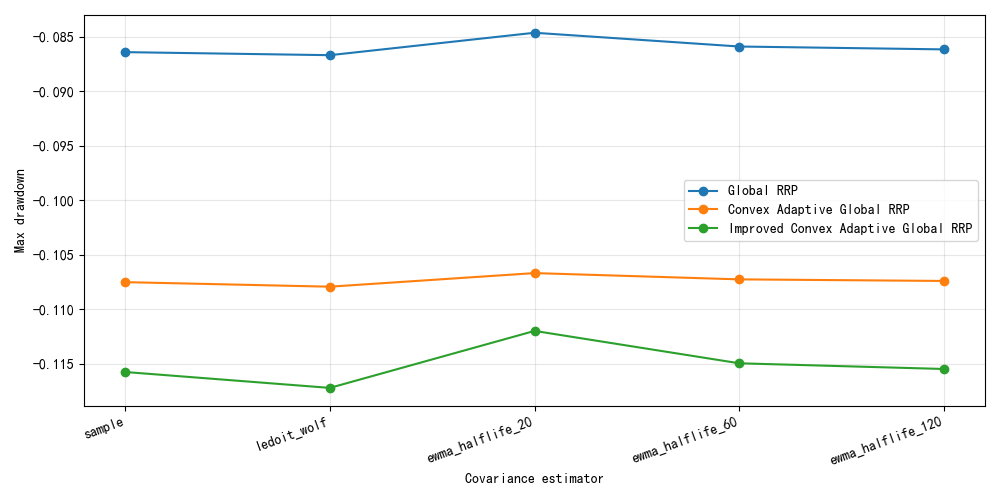
\includegraphics[width=0.88\textwidth]{covariance_robustness_drawdown.png}
  \end{center}
\end{frame}

\begin{frame}{压力期表现}
  \begin{columns}[T]
    \begin{column}{0.50\textwidth}
      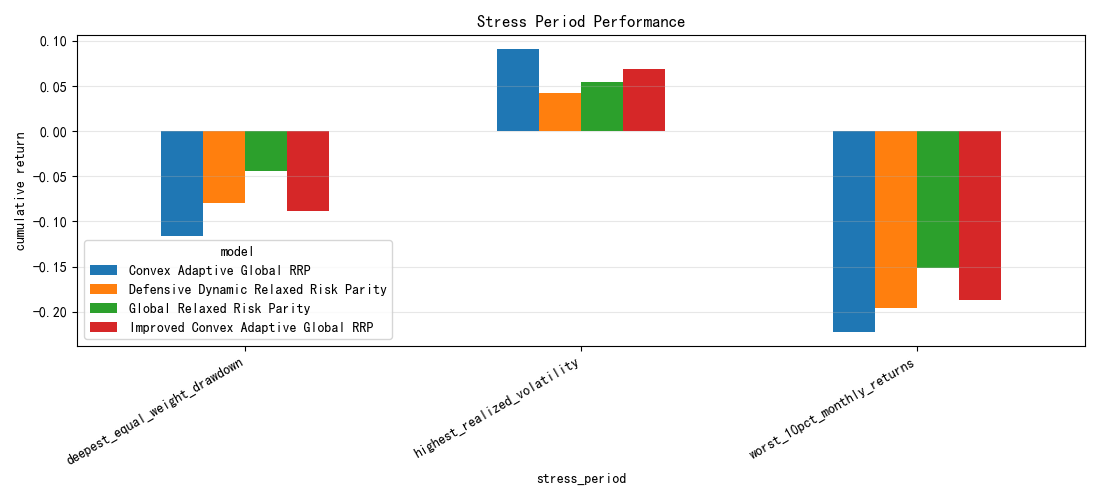
\includegraphics[width=\textwidth]{robustness_stress_period_performance.png}
    \end{column}
    \begin{column}{0.50\textwidth}
      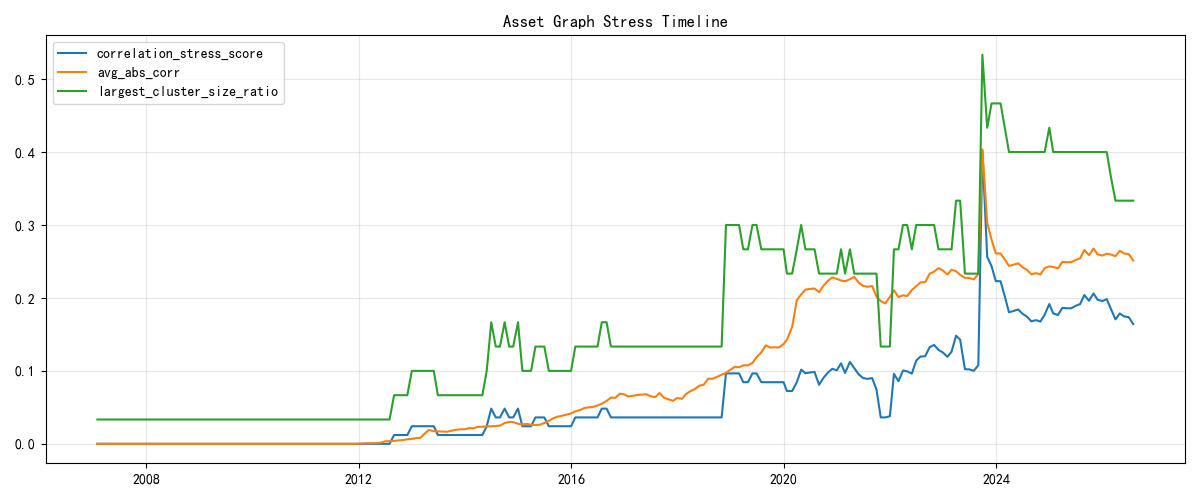
\includegraphics[width=\textwidth]{asset_graph_stress_timeline.png}
    \end{column}
  \end{columns}
\end{frame}

% ════════════════════════════════════════════════════════════════════════════
\section{主要结论}
% ════════════════════════════════════════════════════════════════════════════

\begin{frame}{三条核心结论}
  \begin{swufekeypoints}
    \swufepoint{换手与风险同步改善}{01}{Improved Convex 月换手从 \globalMonthlyTurnover{} 降至 \improvedMonthlyTurnover{}，Sharpe 升至 \improvedSharpe{}，最大回撤收窄至 \improvedMaxDD{}，优势统计显著（$p=\improvedVsGlobalPValue$）}
    \swufepoint{HERC 的高 Sharpe 不具可比性}{02}{HERC 净收益仅 \hercNetReturn{}，年化波动率 0.57\%，来自近乎全仓债券的极低波动，非多资产分散的结果}
    \swufepoint{结论有明确的适用边界}{03}{所有数字条件于 \evalStartDate{}—\evalEndDate{} 特定样本期及冻结参数，Walk-forward 和扰动分析确认区间内相对稳定}
  \end{swufekeypoints}
\end{frame}

\begin{frame}{研究局限与未来方向}
  \begin{columns}[T]
    \begin{column}{0.48\textwidth}
      \textbf{三项局限}
      \begin{enumerate}
        \item 样本期 89 个月，包含低利率→加息周期，与历史长期均值存在偏差
        \item 协方差估计依赖历史数据，快速机制切换时 EWMA 存在滞后
        \item 线性成本近似在大规模执行场景下需精细化
      \end{enumerate}
    \end{column}
    \begin{column}{0.48\textwidth}
      \textbf{未来研究方向}
      \begin{itemize}
        \item 因子层 CVaR 约束（资产 + 因子双层预算）
        \item 机器学习协方差估计器与凸优化结合
        \item 更长历史区间（含 2015 股灾、2020 新冠）
        \item 实盘滑点与冲击成本的精细化建模
      \end{itemize}
    \end{column}
  \end{columns}
\end{frame}

% ════════════════════════════════════════════════════════════════════════════
% ── 致谢与问答 ──────────────────────────────────────────────────────────────
% ════════════════════════════════════════════════════════════════════════════
\begin{frame}[plain]
  \begin{tikzpicture}[remember picture, overlay]
    \fill[swufeDark] (current page.south west) rectangle (current page.north east);
    \foreach \r in {2.5, 3.8, 5.1} {
      \draw[swufeGold, opacity=0.15, line width=0.8pt] (current page.north east) circle(\r cm);
    }
    \fill[swufeGold] (current page.south west) rectangle ([yshift=6pt]current page.south east);
    \node[text=white, font=\Large\bfseries] at ([yshift=0.5cm]current page.center)
      {感谢各位老师的聆听与指导};
    \node[text=swufeGold, font=\normalsize] at ([yshift=-0.3cm]current page.center)
      {敬请批评指正};
    \node[text=white!70, font=\scriptsize, anchor=south east]
      at ([xshift=-1.5cm, yshift=1.5cm]current page.south east) {
      \begin{tabular}{rl}
        净年化收益 & \improvedNetReturn \\
        Sharpe    & \improvedSharpe \\
        最大回撤  & \improvedMaxDD \\
        月均换手  & \improvedMonthlyTurnover \\
      \end{tabular}
    };
    \node[anchor=north west, opacity=0.6]
      at ([xshift=1cm, yshift=-0.8cm]current page.north west) {
      
\includegraphics[height=1.2cm]{logo.png}
    };
  \end{tikzpicture}
\end{frame}

\end{document}
